\cleardoublepage
\section{Example tutorial case results}
\label{sec:exp}

In the present section the results of the chosen example tutorial case are presented. The simulation of the flow, and the air pollution spreading are performed in the segregated manner. 

Firstly, we focus onto the flow results, i.e.\ the solution of~(\ref{eq:RANS1},~\ref{eq:RANS2}). The simulation run in parallel utilizing 12 cores of the Taiwania-3 server~\cite{tw3} for approximately 4 hours.  The resulting stream-wise velocity component contours ($u_x$) on the $y$-normal slice, and the pressure contours ($p$) on the ground computational domain boundary ($\partial\Omega_{\mathrm{g}}$) are presented in Figure~\ref{fig:ux_p}a. 

\begin{figure}[htpb]
    \begin{tikzpicture}
        \node (up) {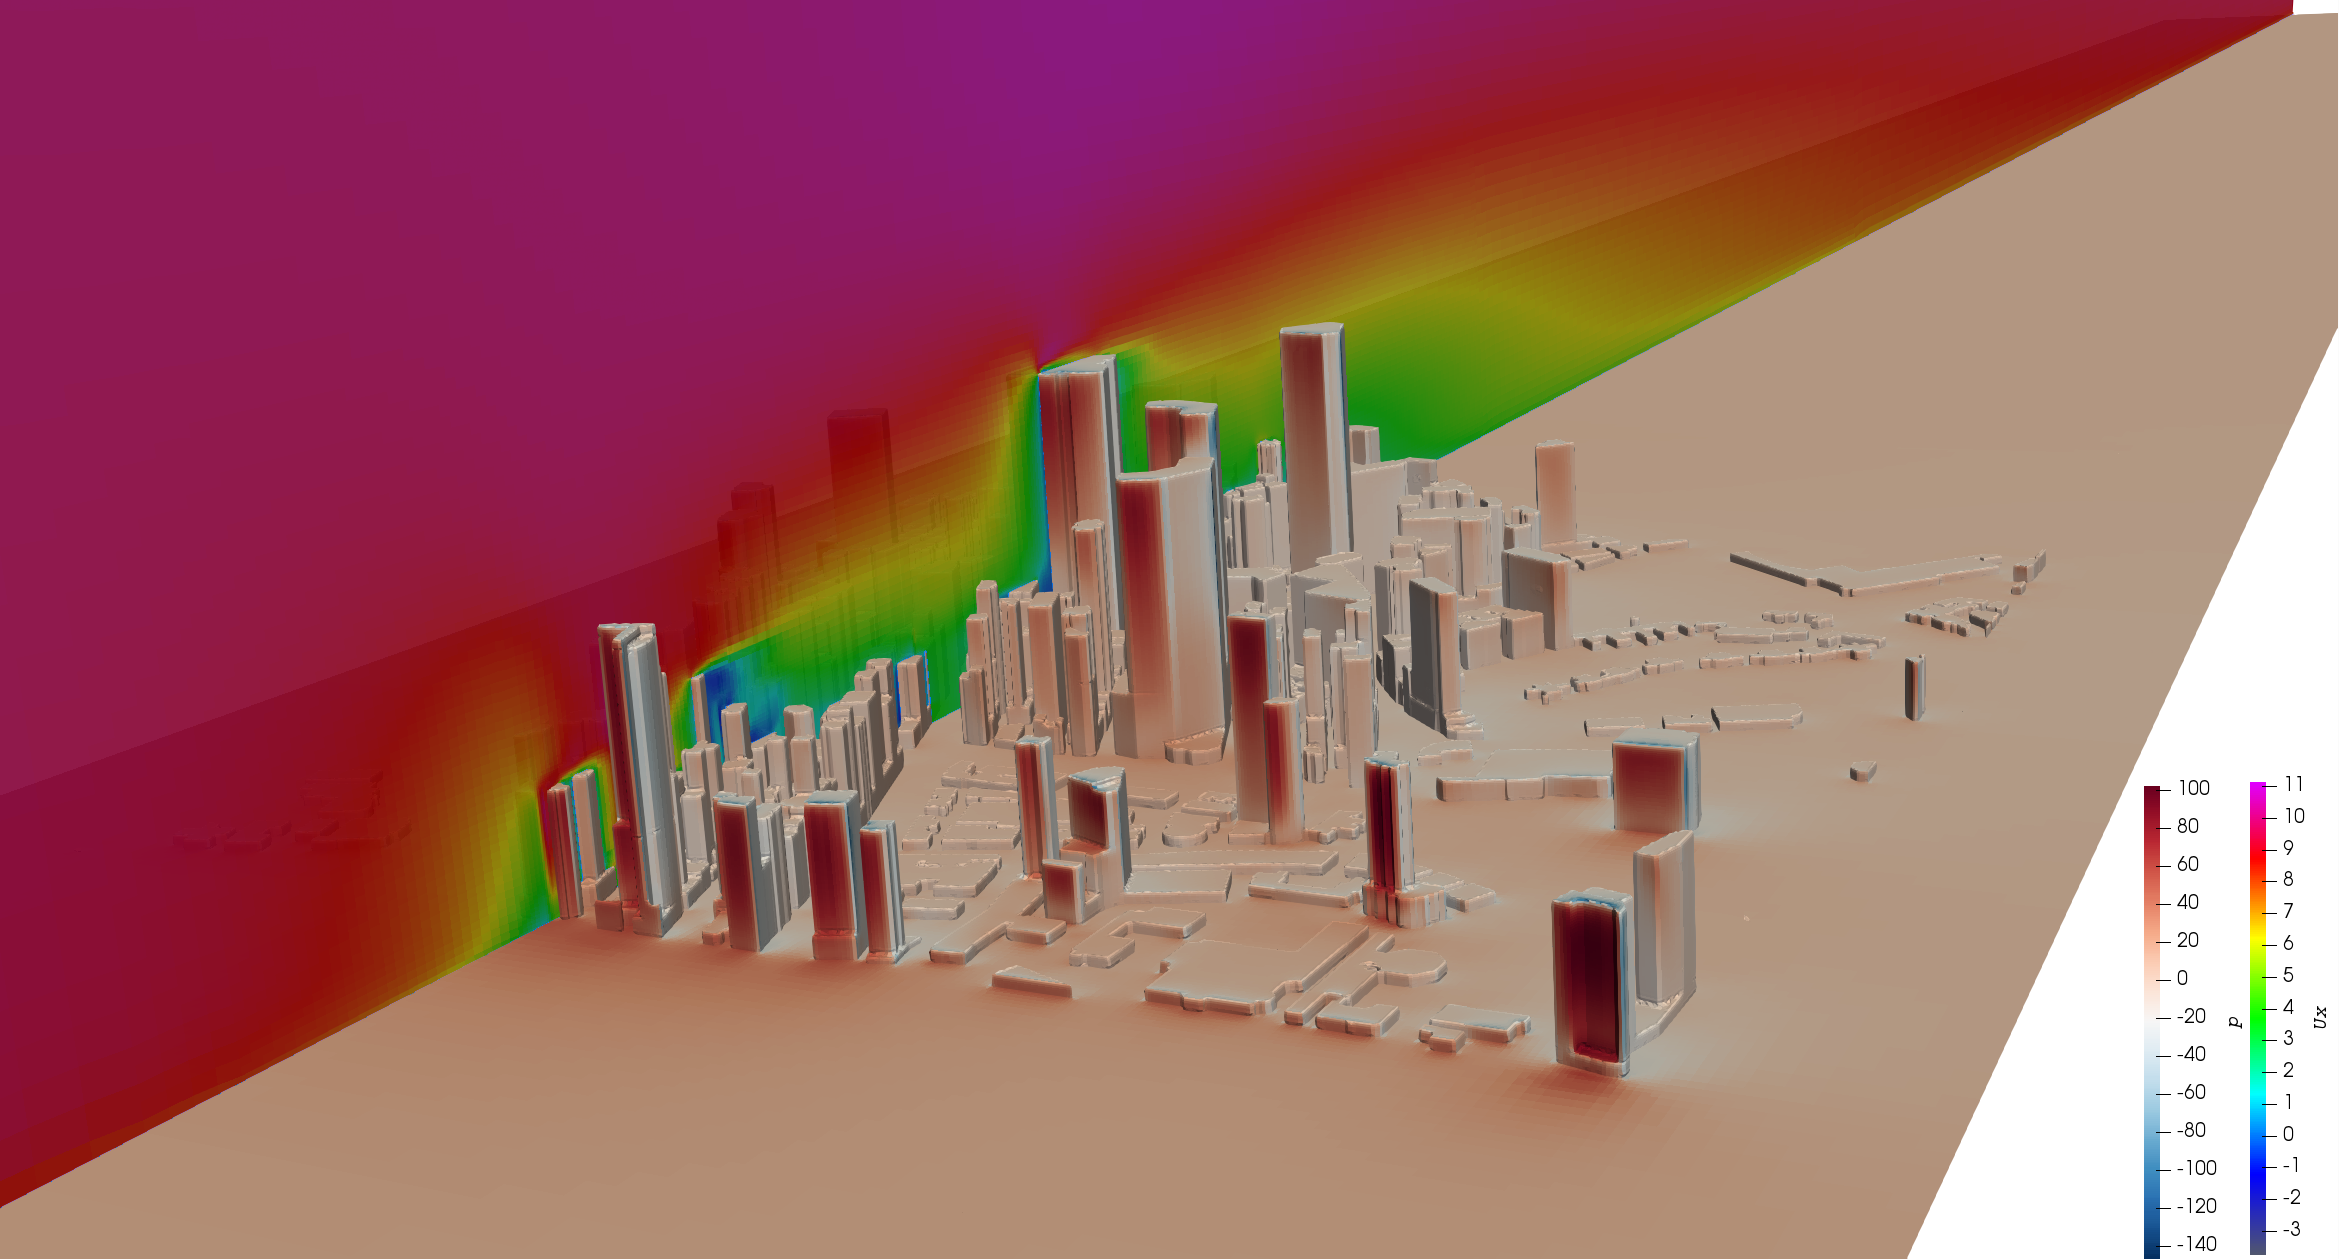
\includegraphics[width=0.95\textwidth]{01_images/res/pUxFront2.png}};
        \node at (up.north west) [anchor=north west, color=white, shift={(0.2cm,0-0.2cm)}] {a)}; 
        \node (down) at (up.south) [anchor=north] {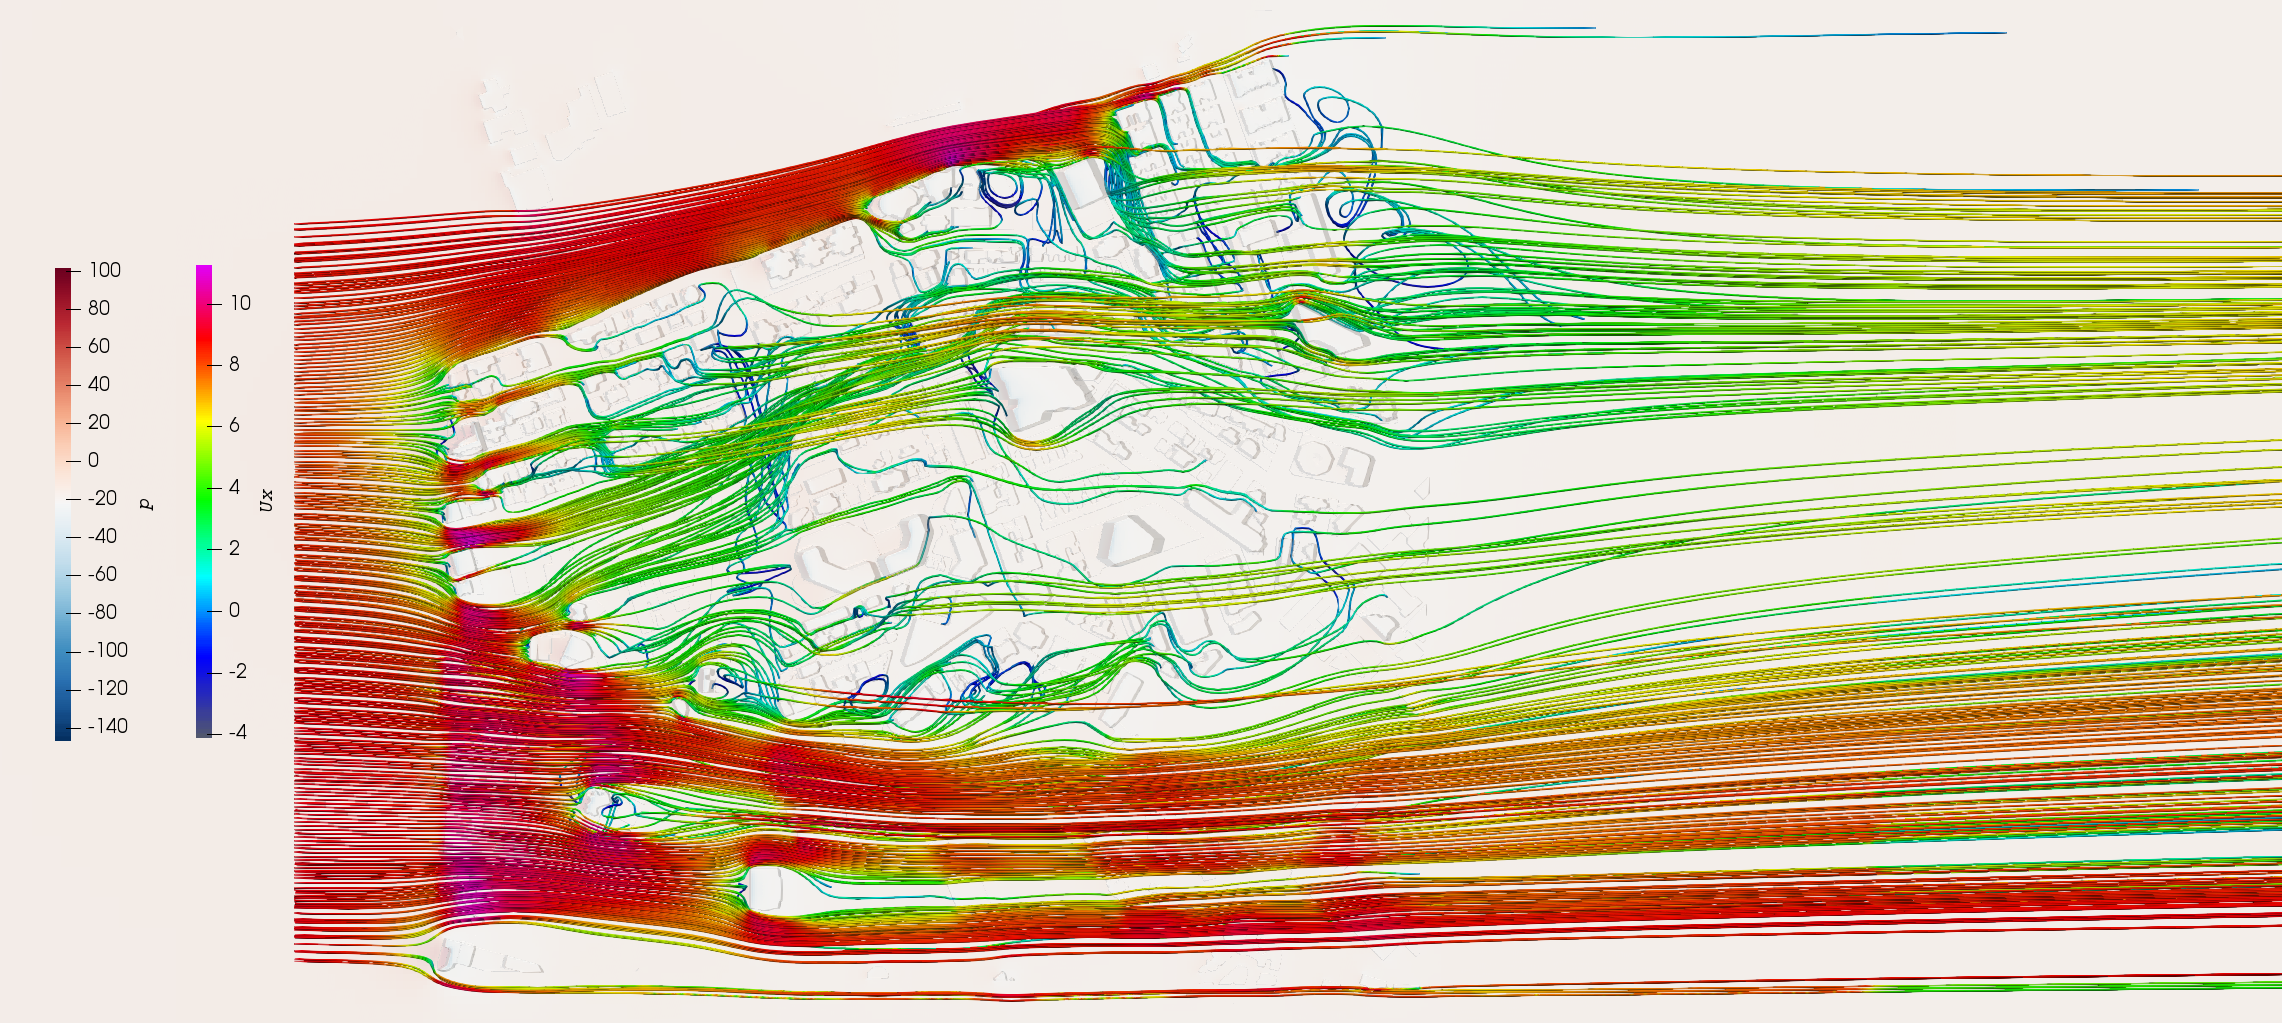
\includegraphics[width=0.95\textwidth]{01_images/res/streamUp2.png}};
        \node at (down.north west) [anchor=north west,shift={(0.2cm,0-0.2cm)}] {b)};
    \end{tikzpicture}
    
    \caption{a) Stream-vise velocity component ($u_x$), and pressure ($p$) contours on $y$-normal slice, and the ground boundary, respectively, b) main flow pathways visualized using flow streamlines colored by streamwise velocity component.}
    \label{fig:ux_p}
\end{figure}

\begin{figure}[htpb]
    \begin{tikzpicture}
        \node (left) {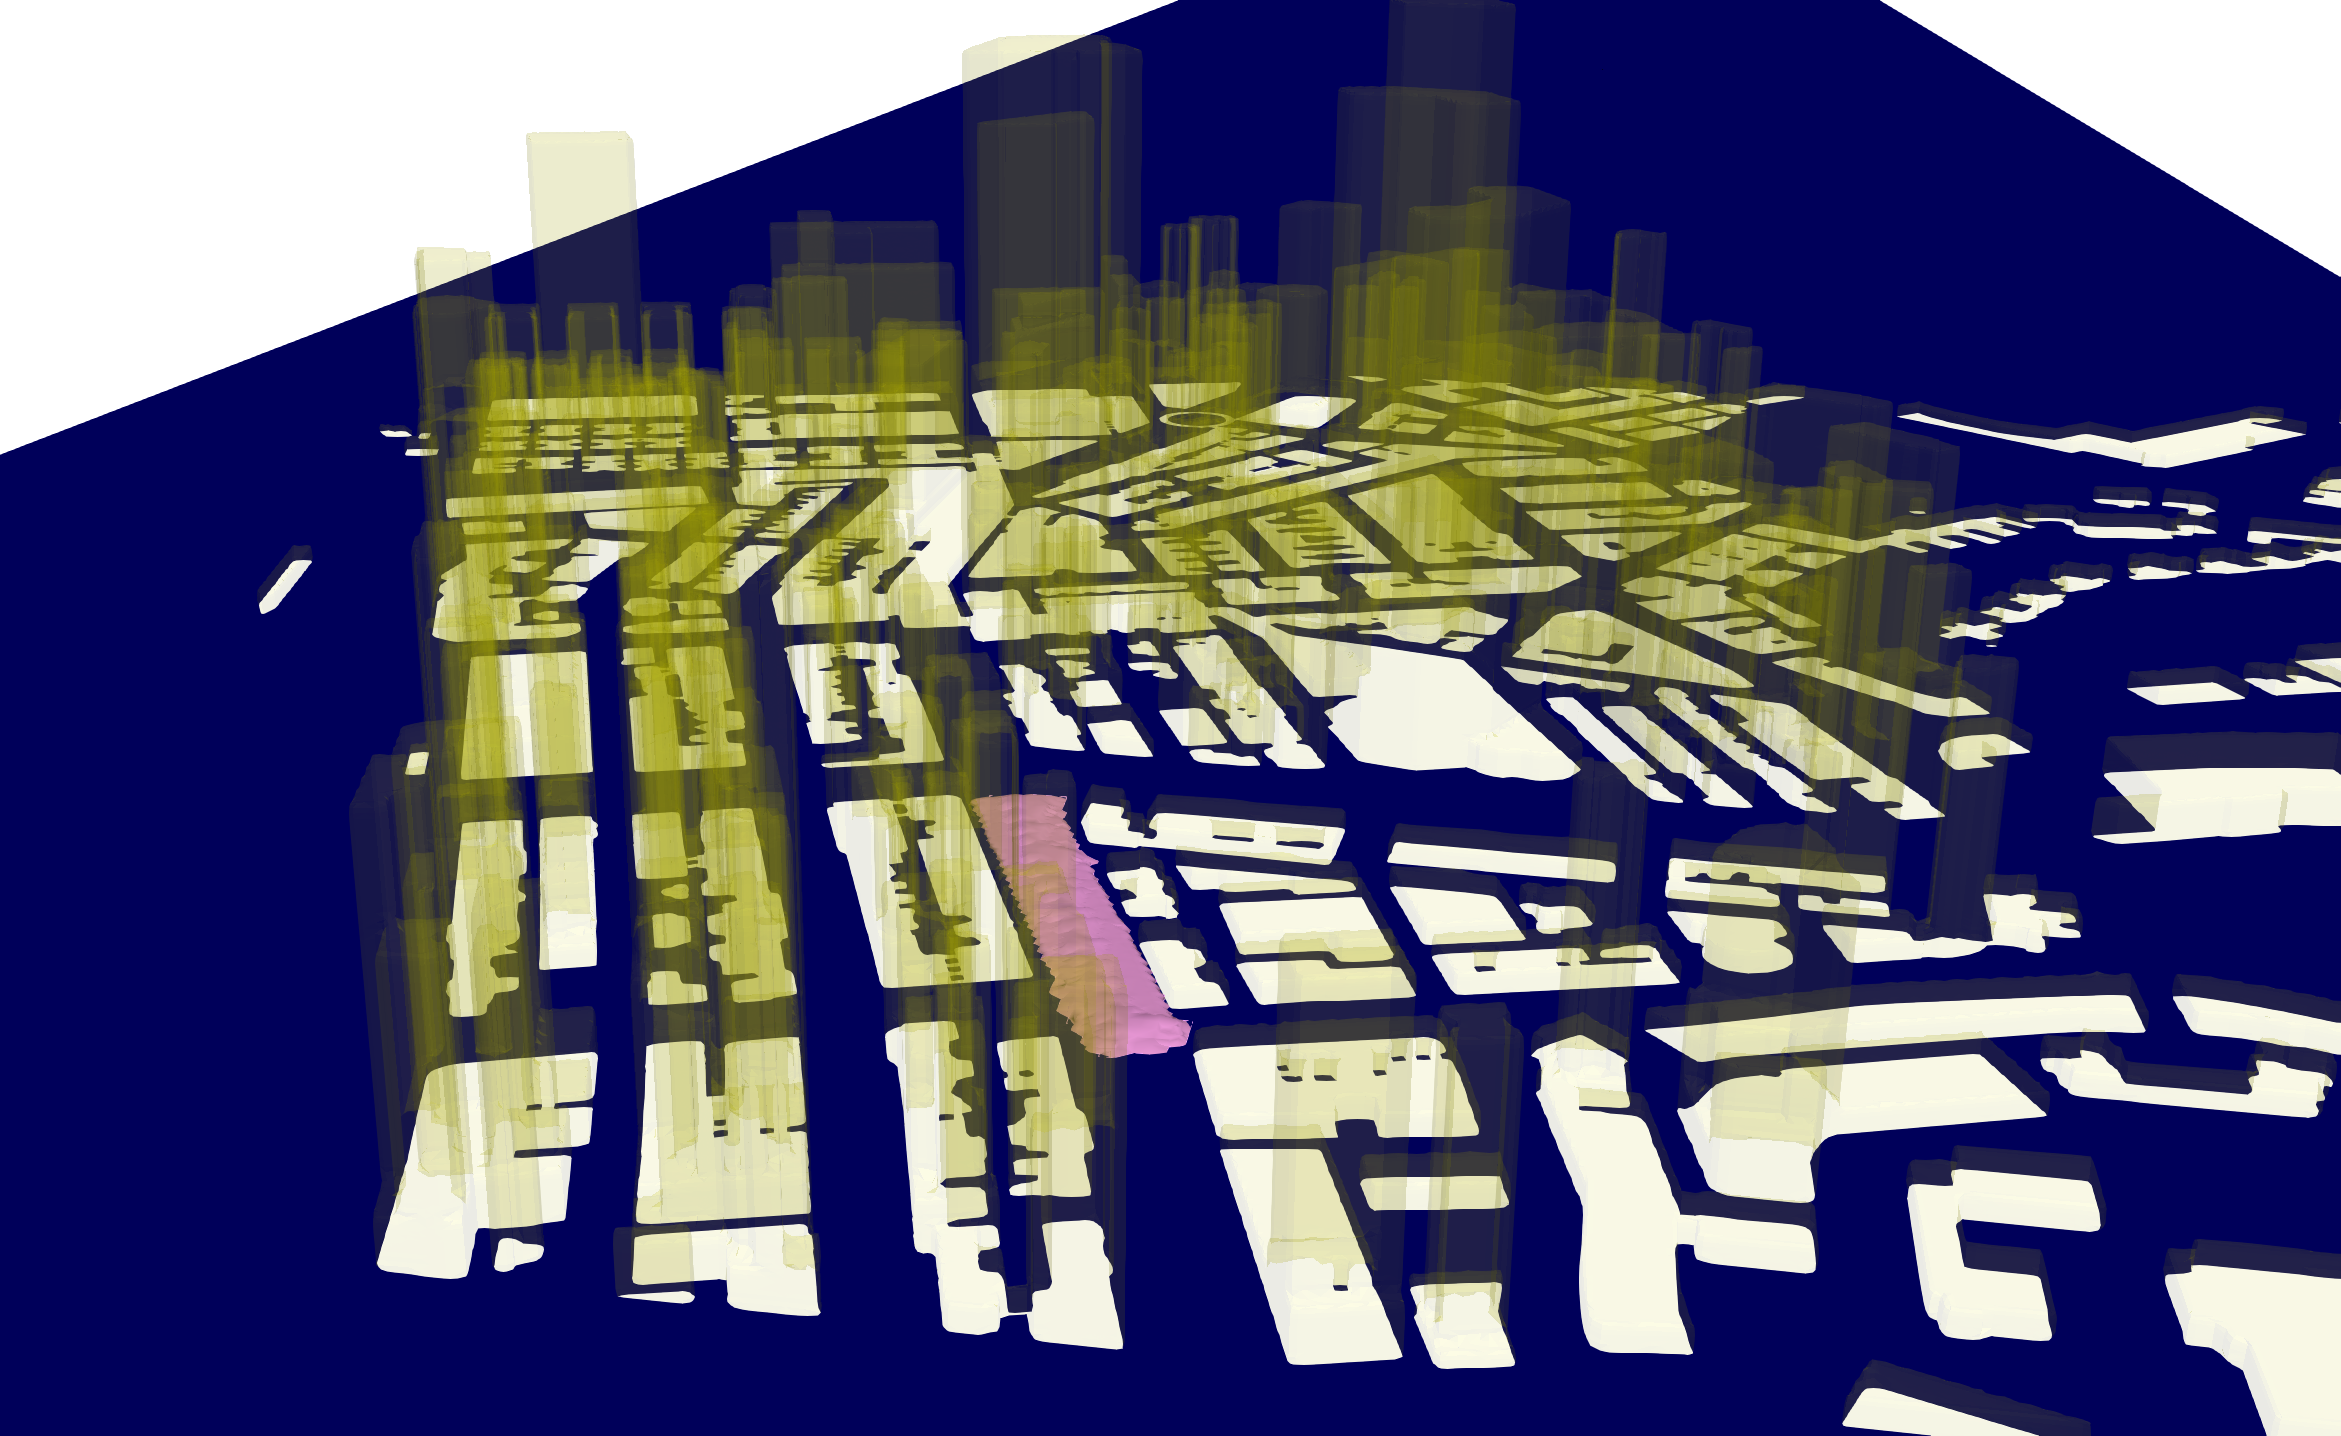
\includegraphics[width = 0.5\textwidth, trim={0 50px 0 200px},clip]{01_images/anim/animV1.0002.png}};
        \node at (left.west) [anchor=north, xshift = 0.2cm, rotate=90, color=white] {$t$ = 1\,s};
        % \node (right) at (left.east) [anchor=west] {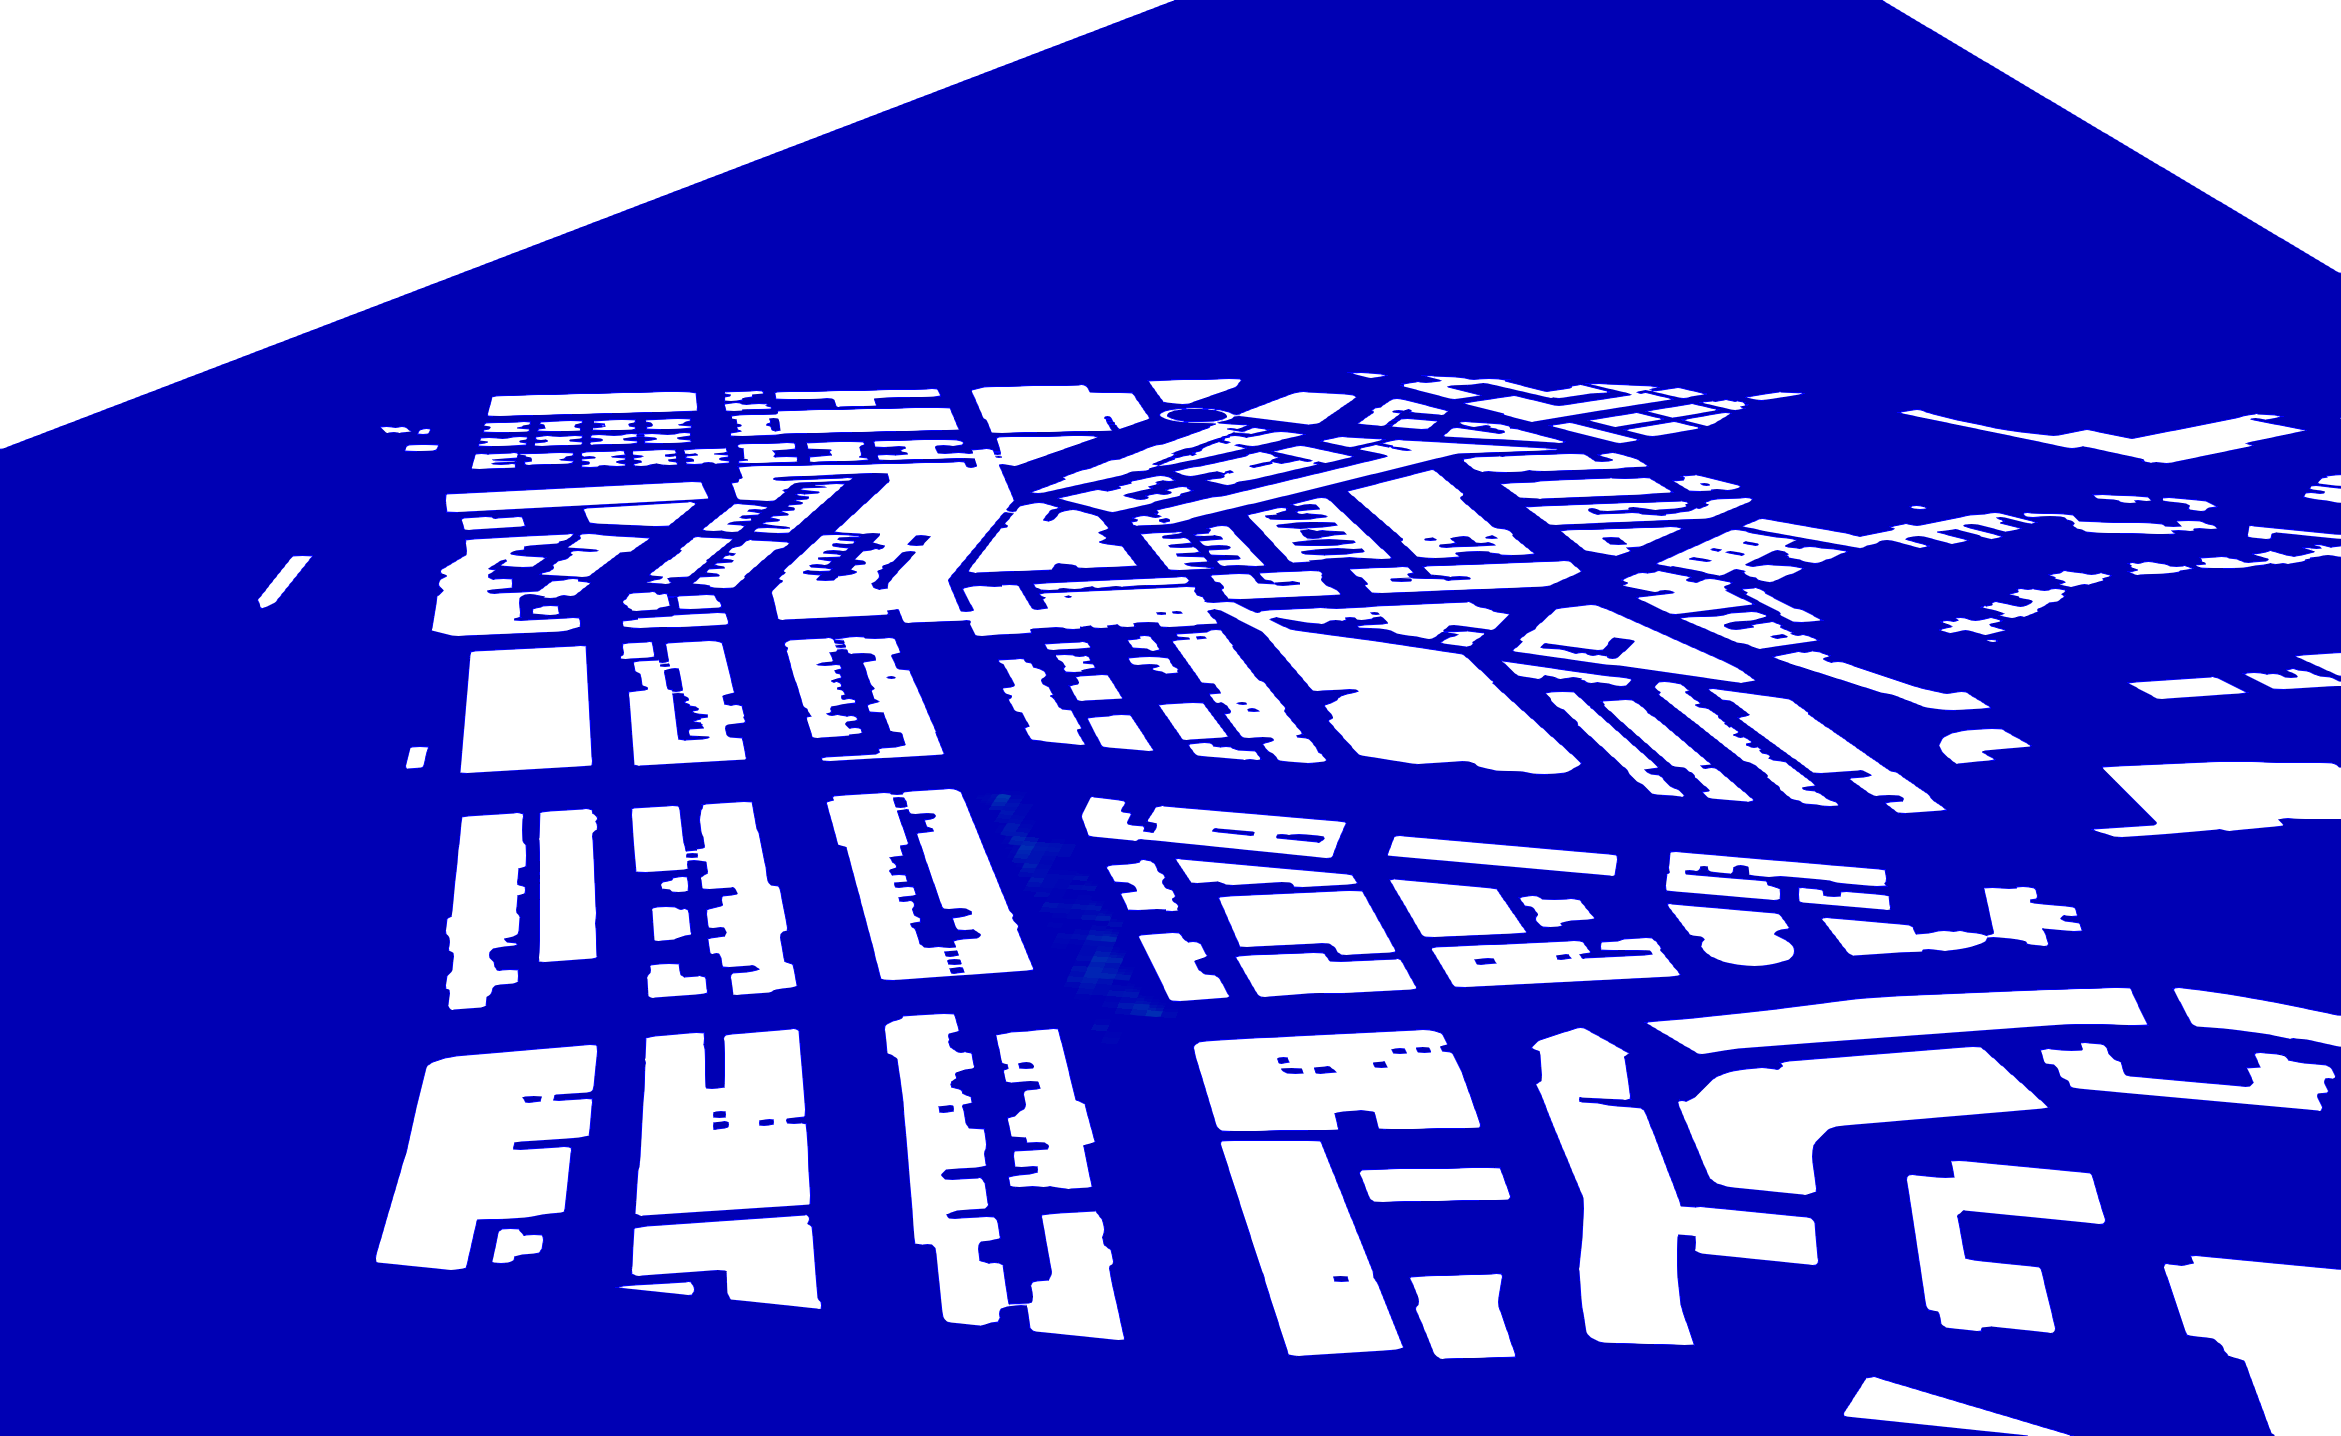
\includegraphics[width=0.23\textwidth, trim={500px 50px 1000px 200px},clip]{01_images/anim2/animV1.0002.png}};
        \node (right) at (left.east) [anchor=west] {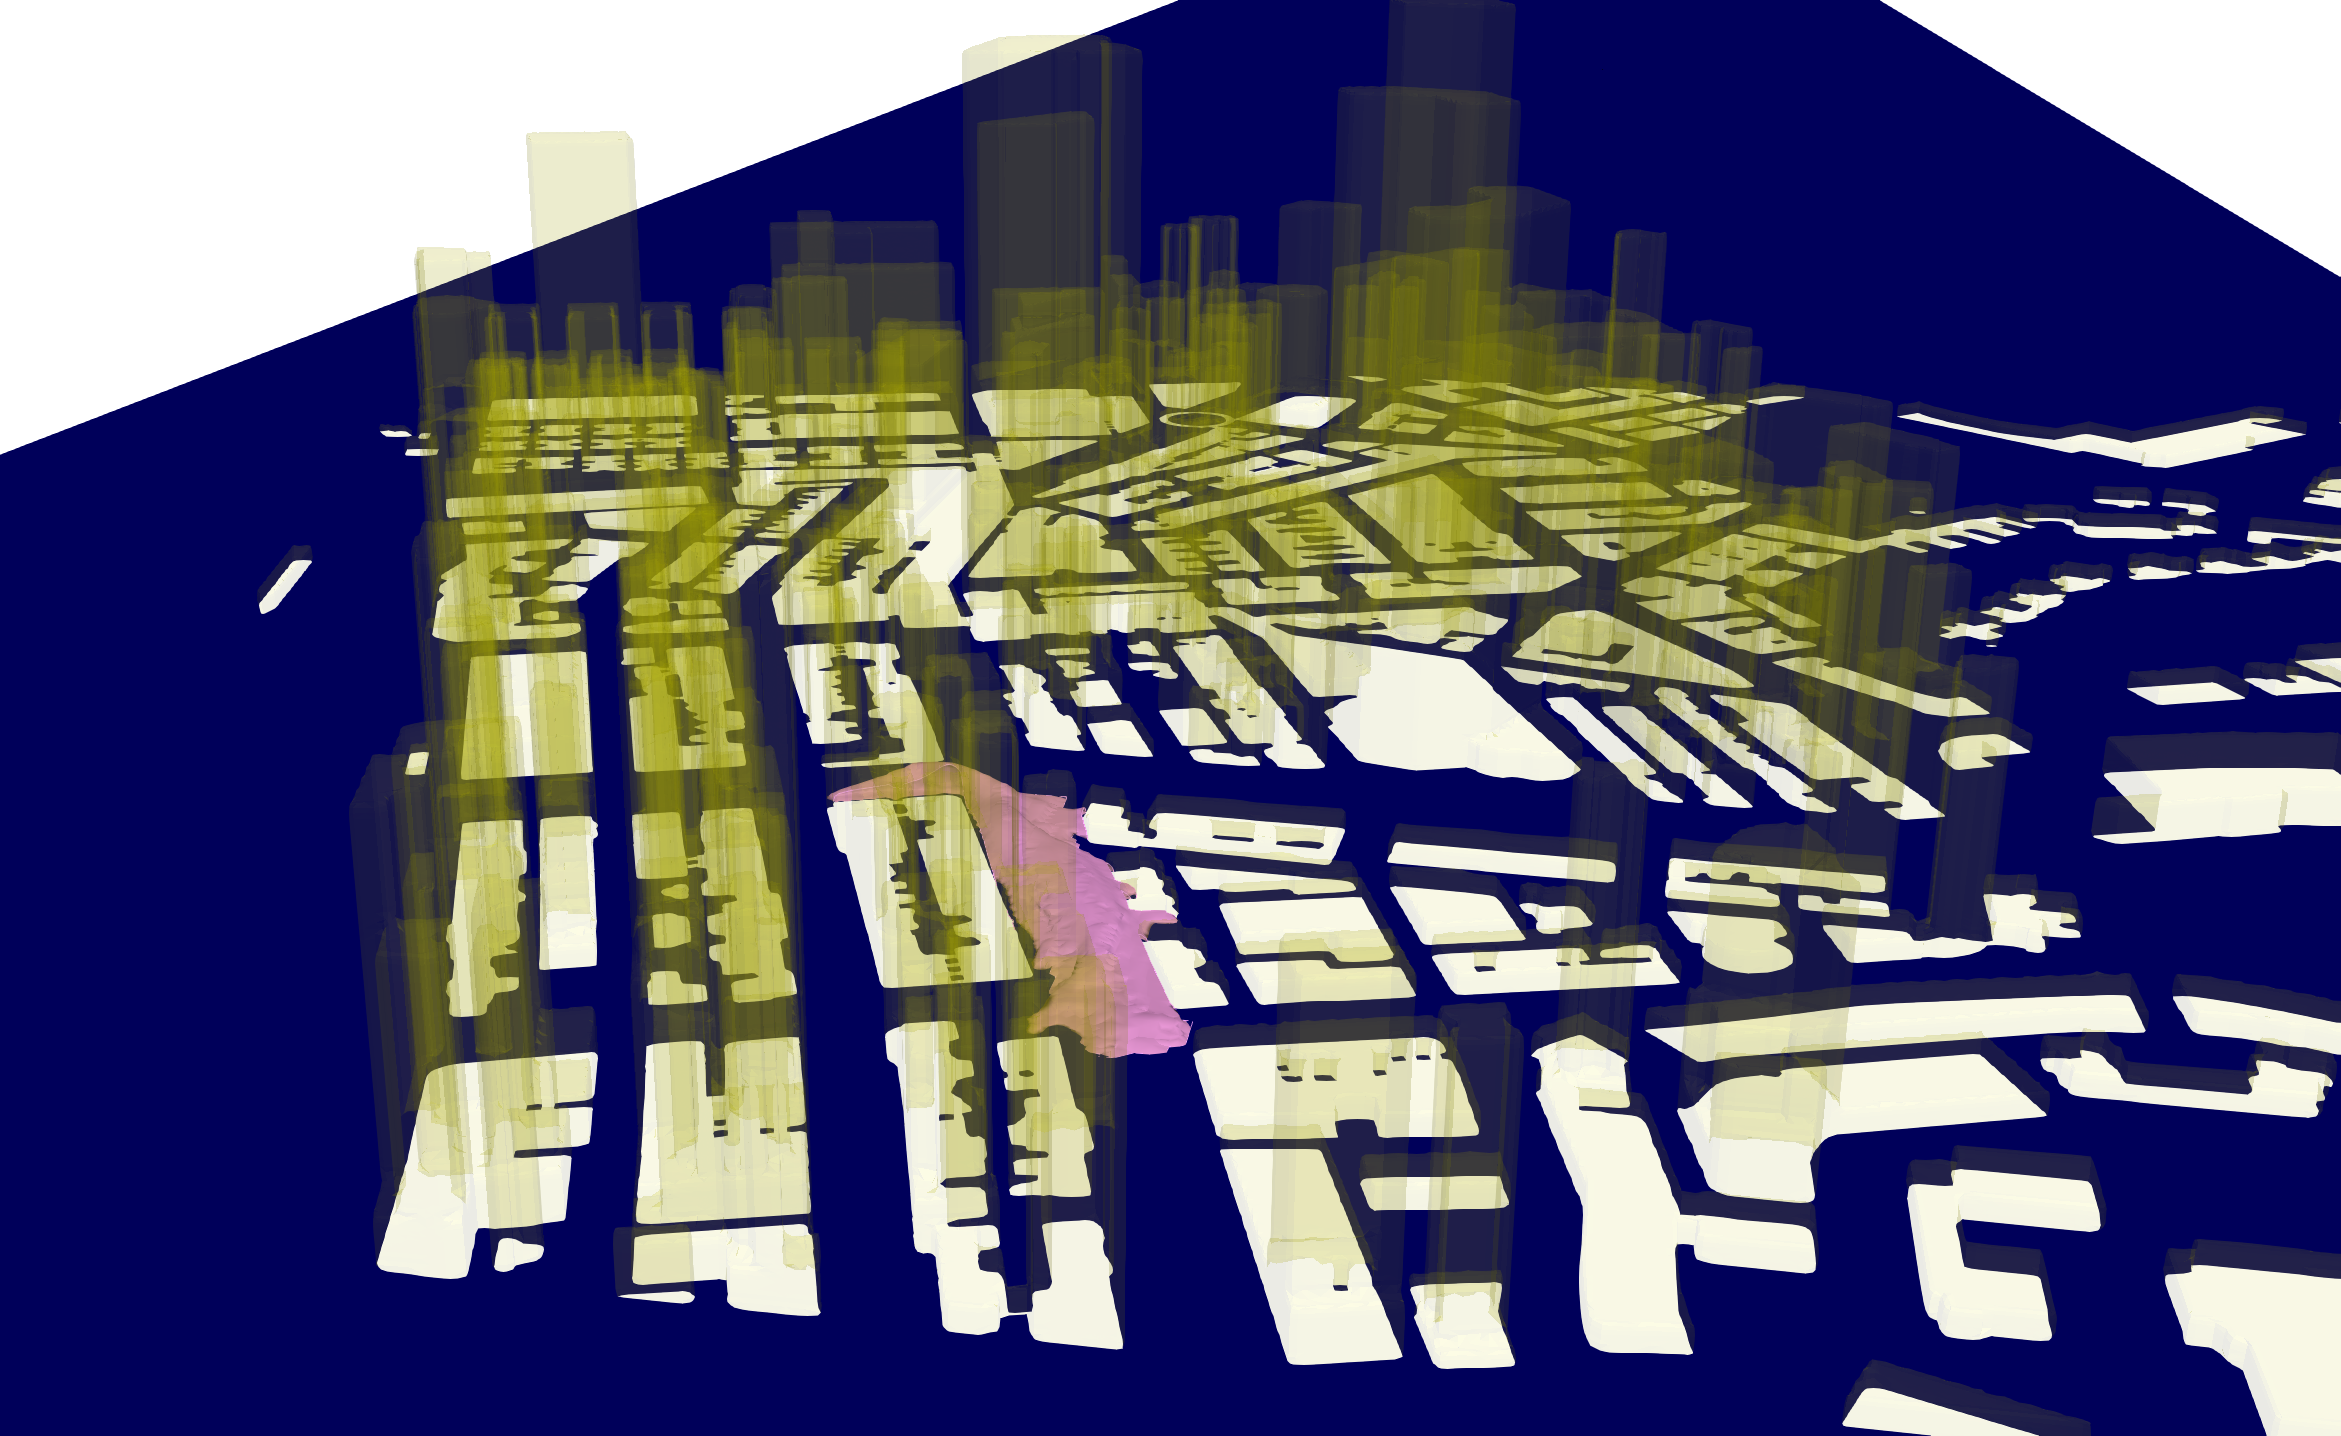
\includegraphics[width = 0.5\textwidth, trim={0 50px 0 200px},clip]{01_images/anim/animV1.0003.png}};
        \node at (right.west) [anchor=north, xshift = 0.2cm, rotate=90, color=white] {$t$ = 10\,s};
        \node (left) at (left.south) [anchor=north] {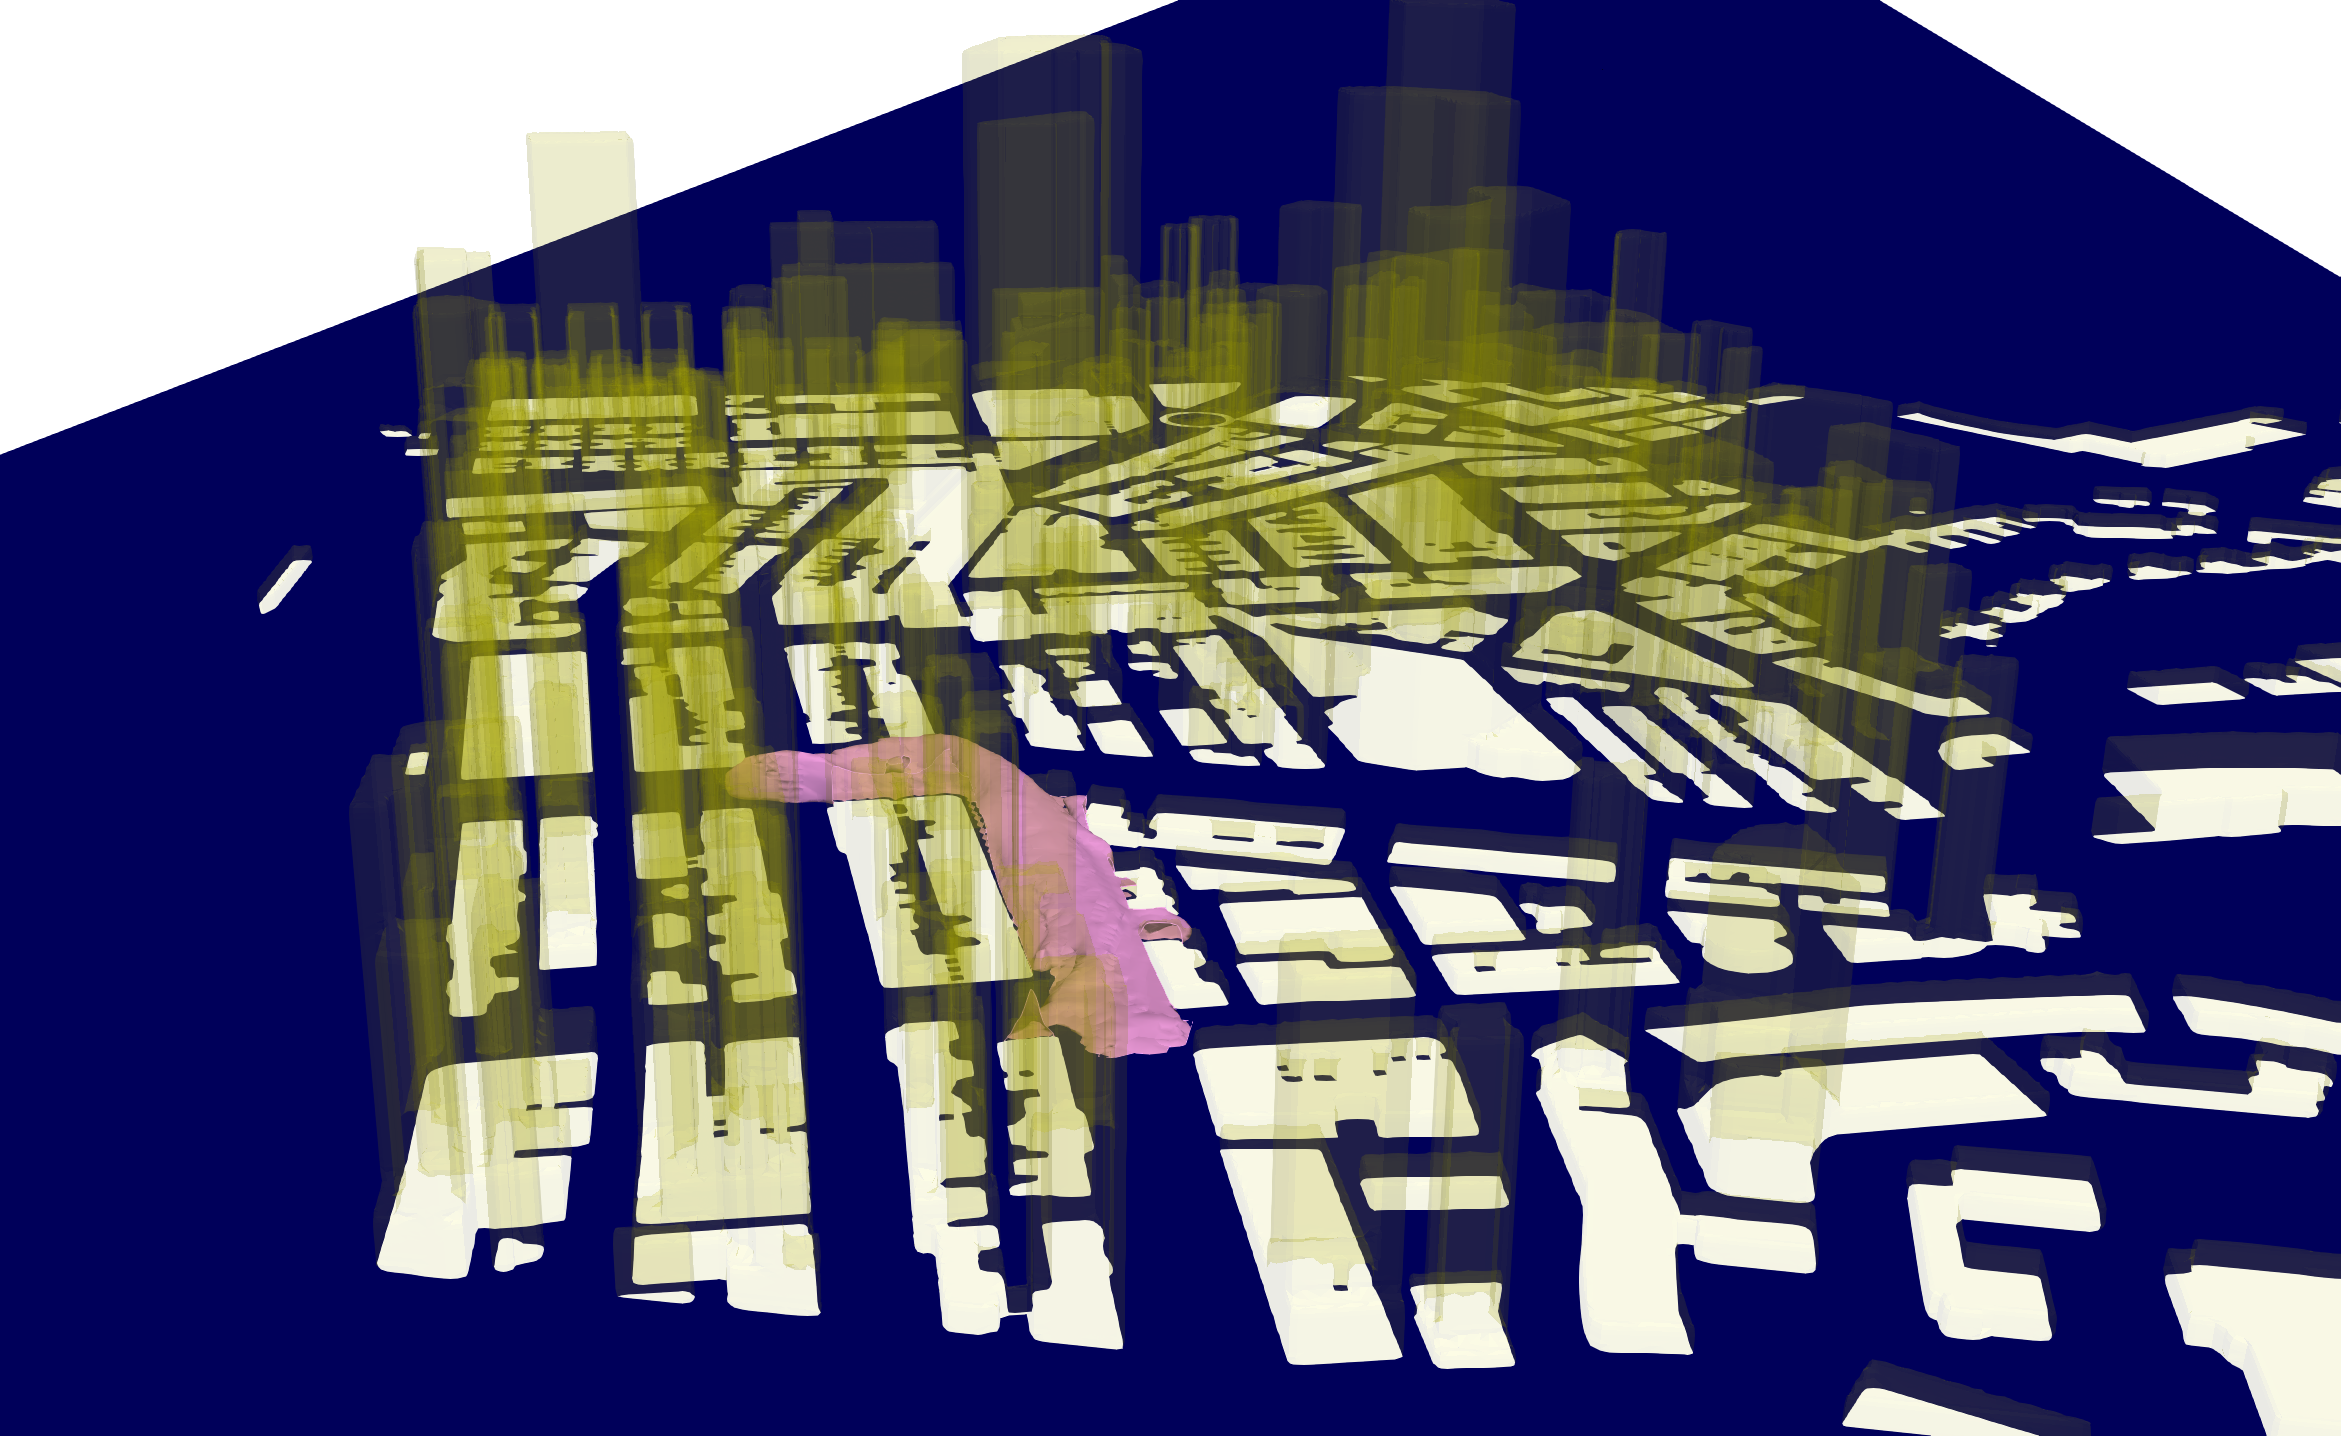
\includegraphics[width = 0.5\textwidth, trim={0 50px 0 200px},clip]{01_images/anim/animV1.0004.png}};
        \node at (left.west) [anchor=north, xshift = 0.2cm, rotate=90, color=white] {$t$ = 20\,s};
        \node (right) at (left.east) [anchor=west] {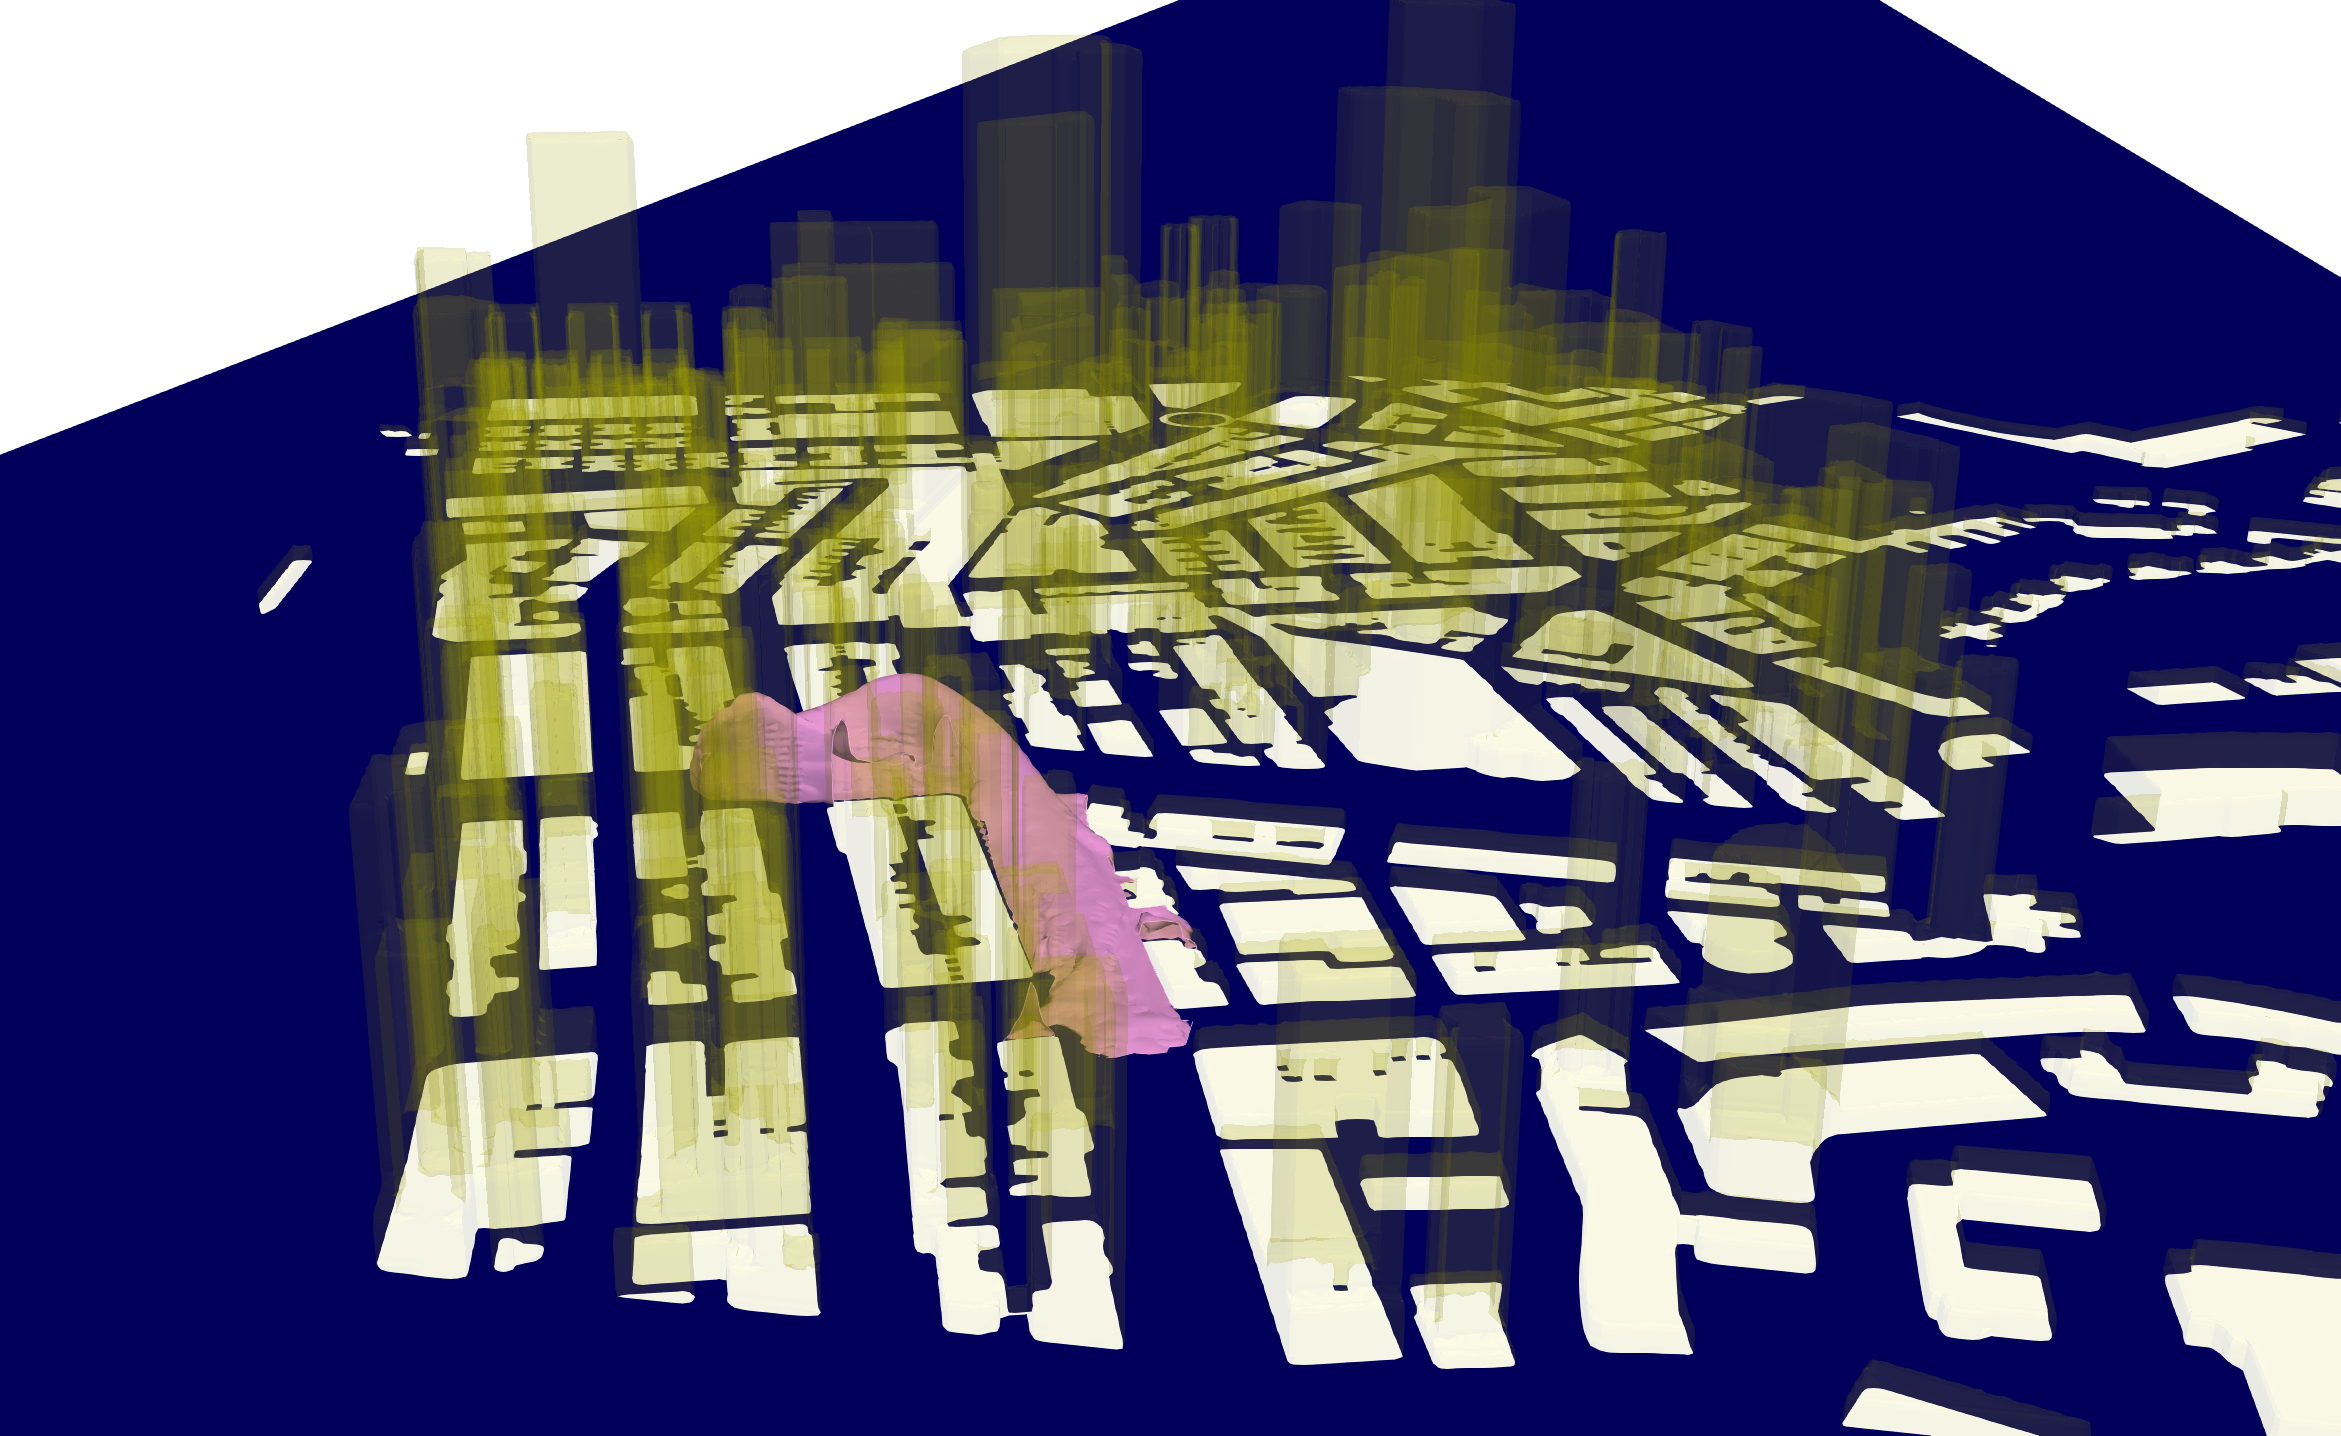
\includegraphics[width = 0.5\textwidth, trim={0 50px 0 200px},clip]{01_images/anim/animV1.0005.png}};
        \node at (right.west) [anchor=north, xshift = 0.2cm, rotate=90, color=white] {$t$ = 30\,s};
        % \node (right) at (left.east) [anchor=west] {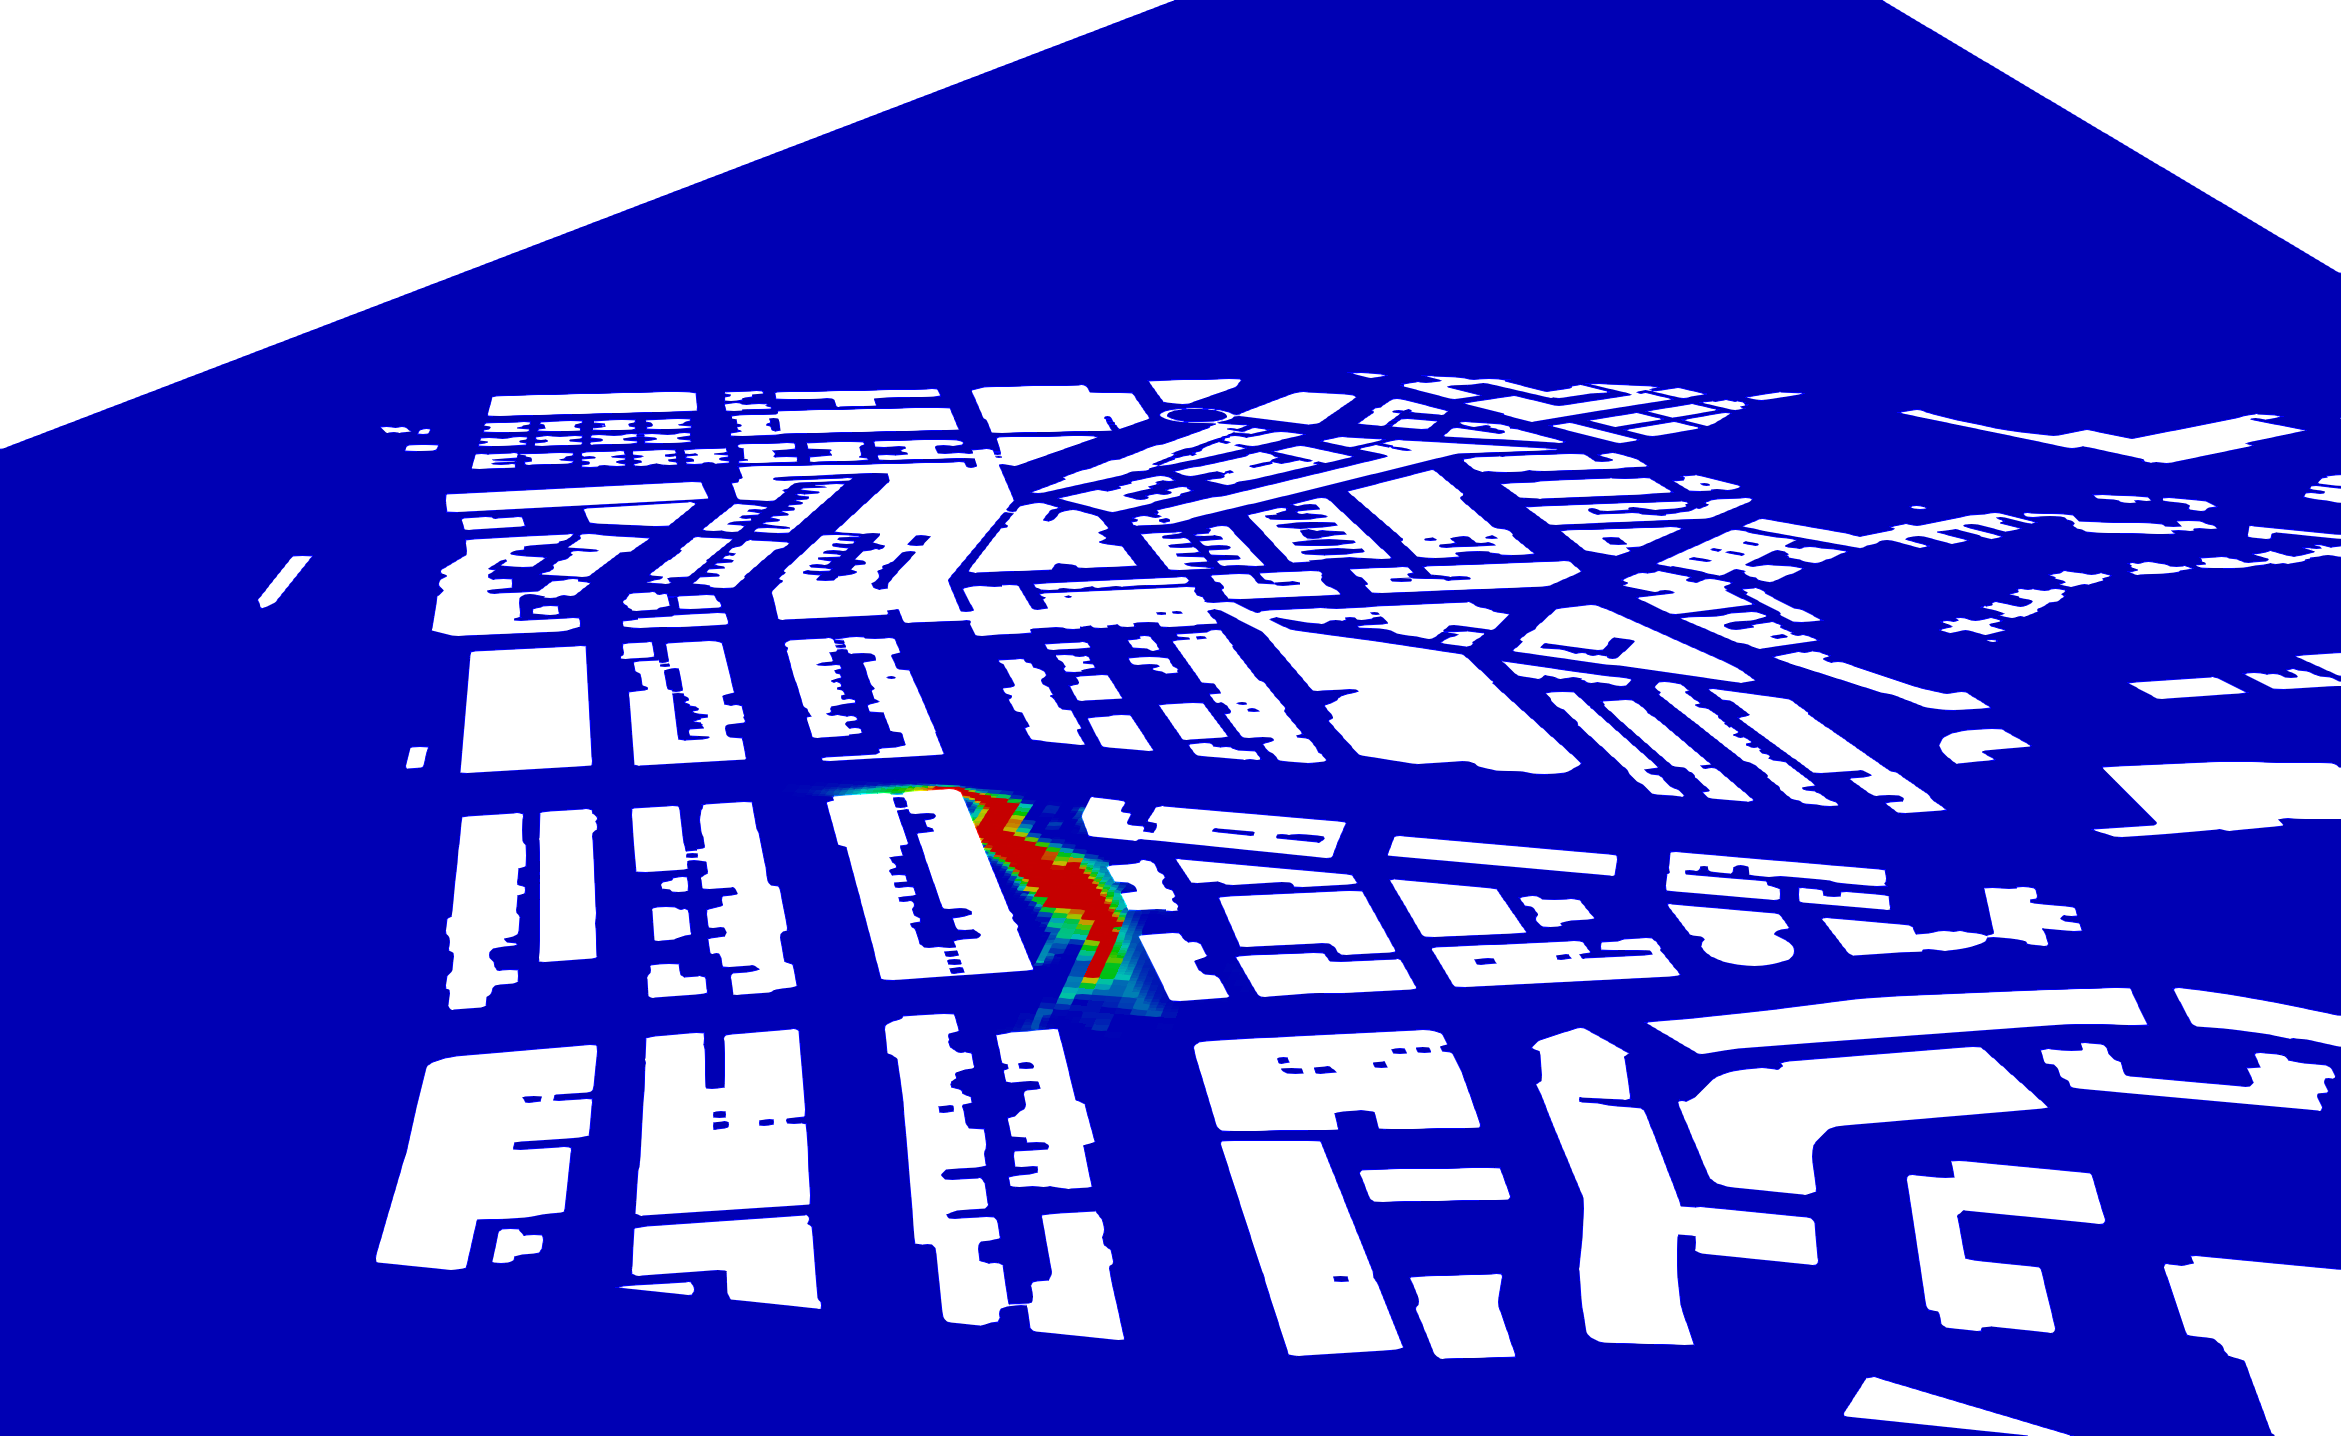
\includegraphics[width=0.23\textwidth, trim={500px 50px 1000px 200px},clip]{01_images/anim2/animV1.0003.png}};
        \node (left) at (left.south) [anchor=north] {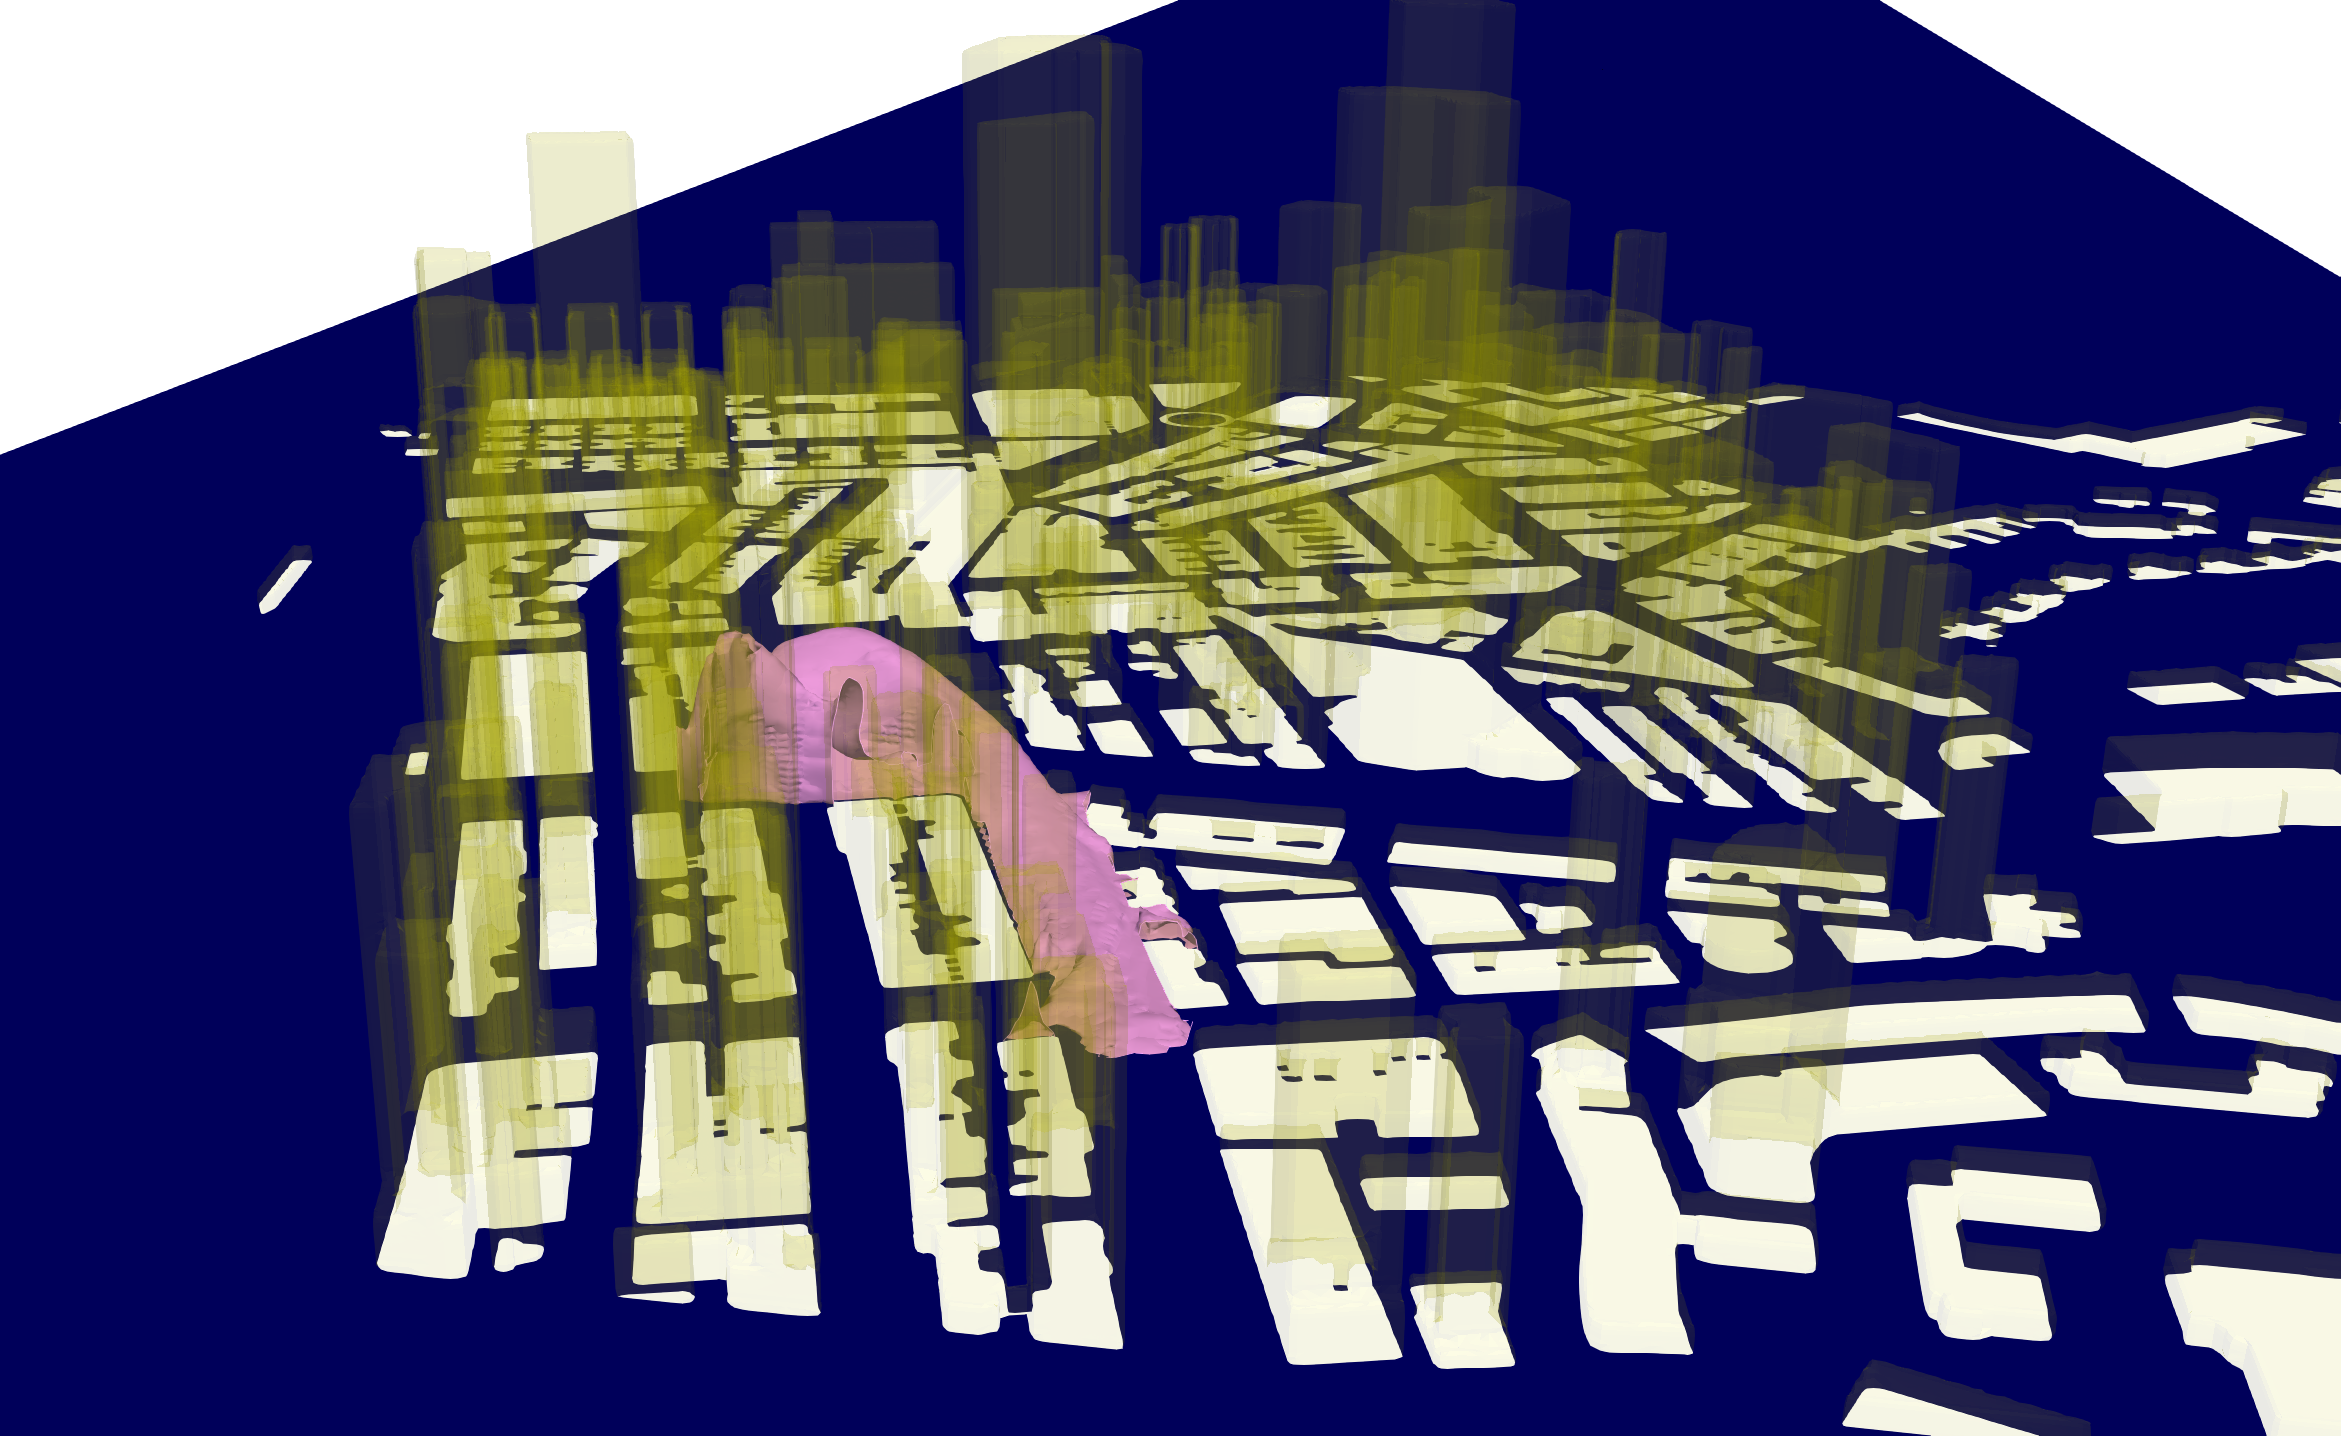
\includegraphics[width = 0.5\textwidth, trim={0 50px 0 200px},clip]{01_images/anim/animV1.0006.png}};
        \node at (left.west) [anchor=north, xshift = 0.2cm, rotate=90, color=white] {$t$ = 40\,s};
        \node (right) at (left.east) [anchor=west] {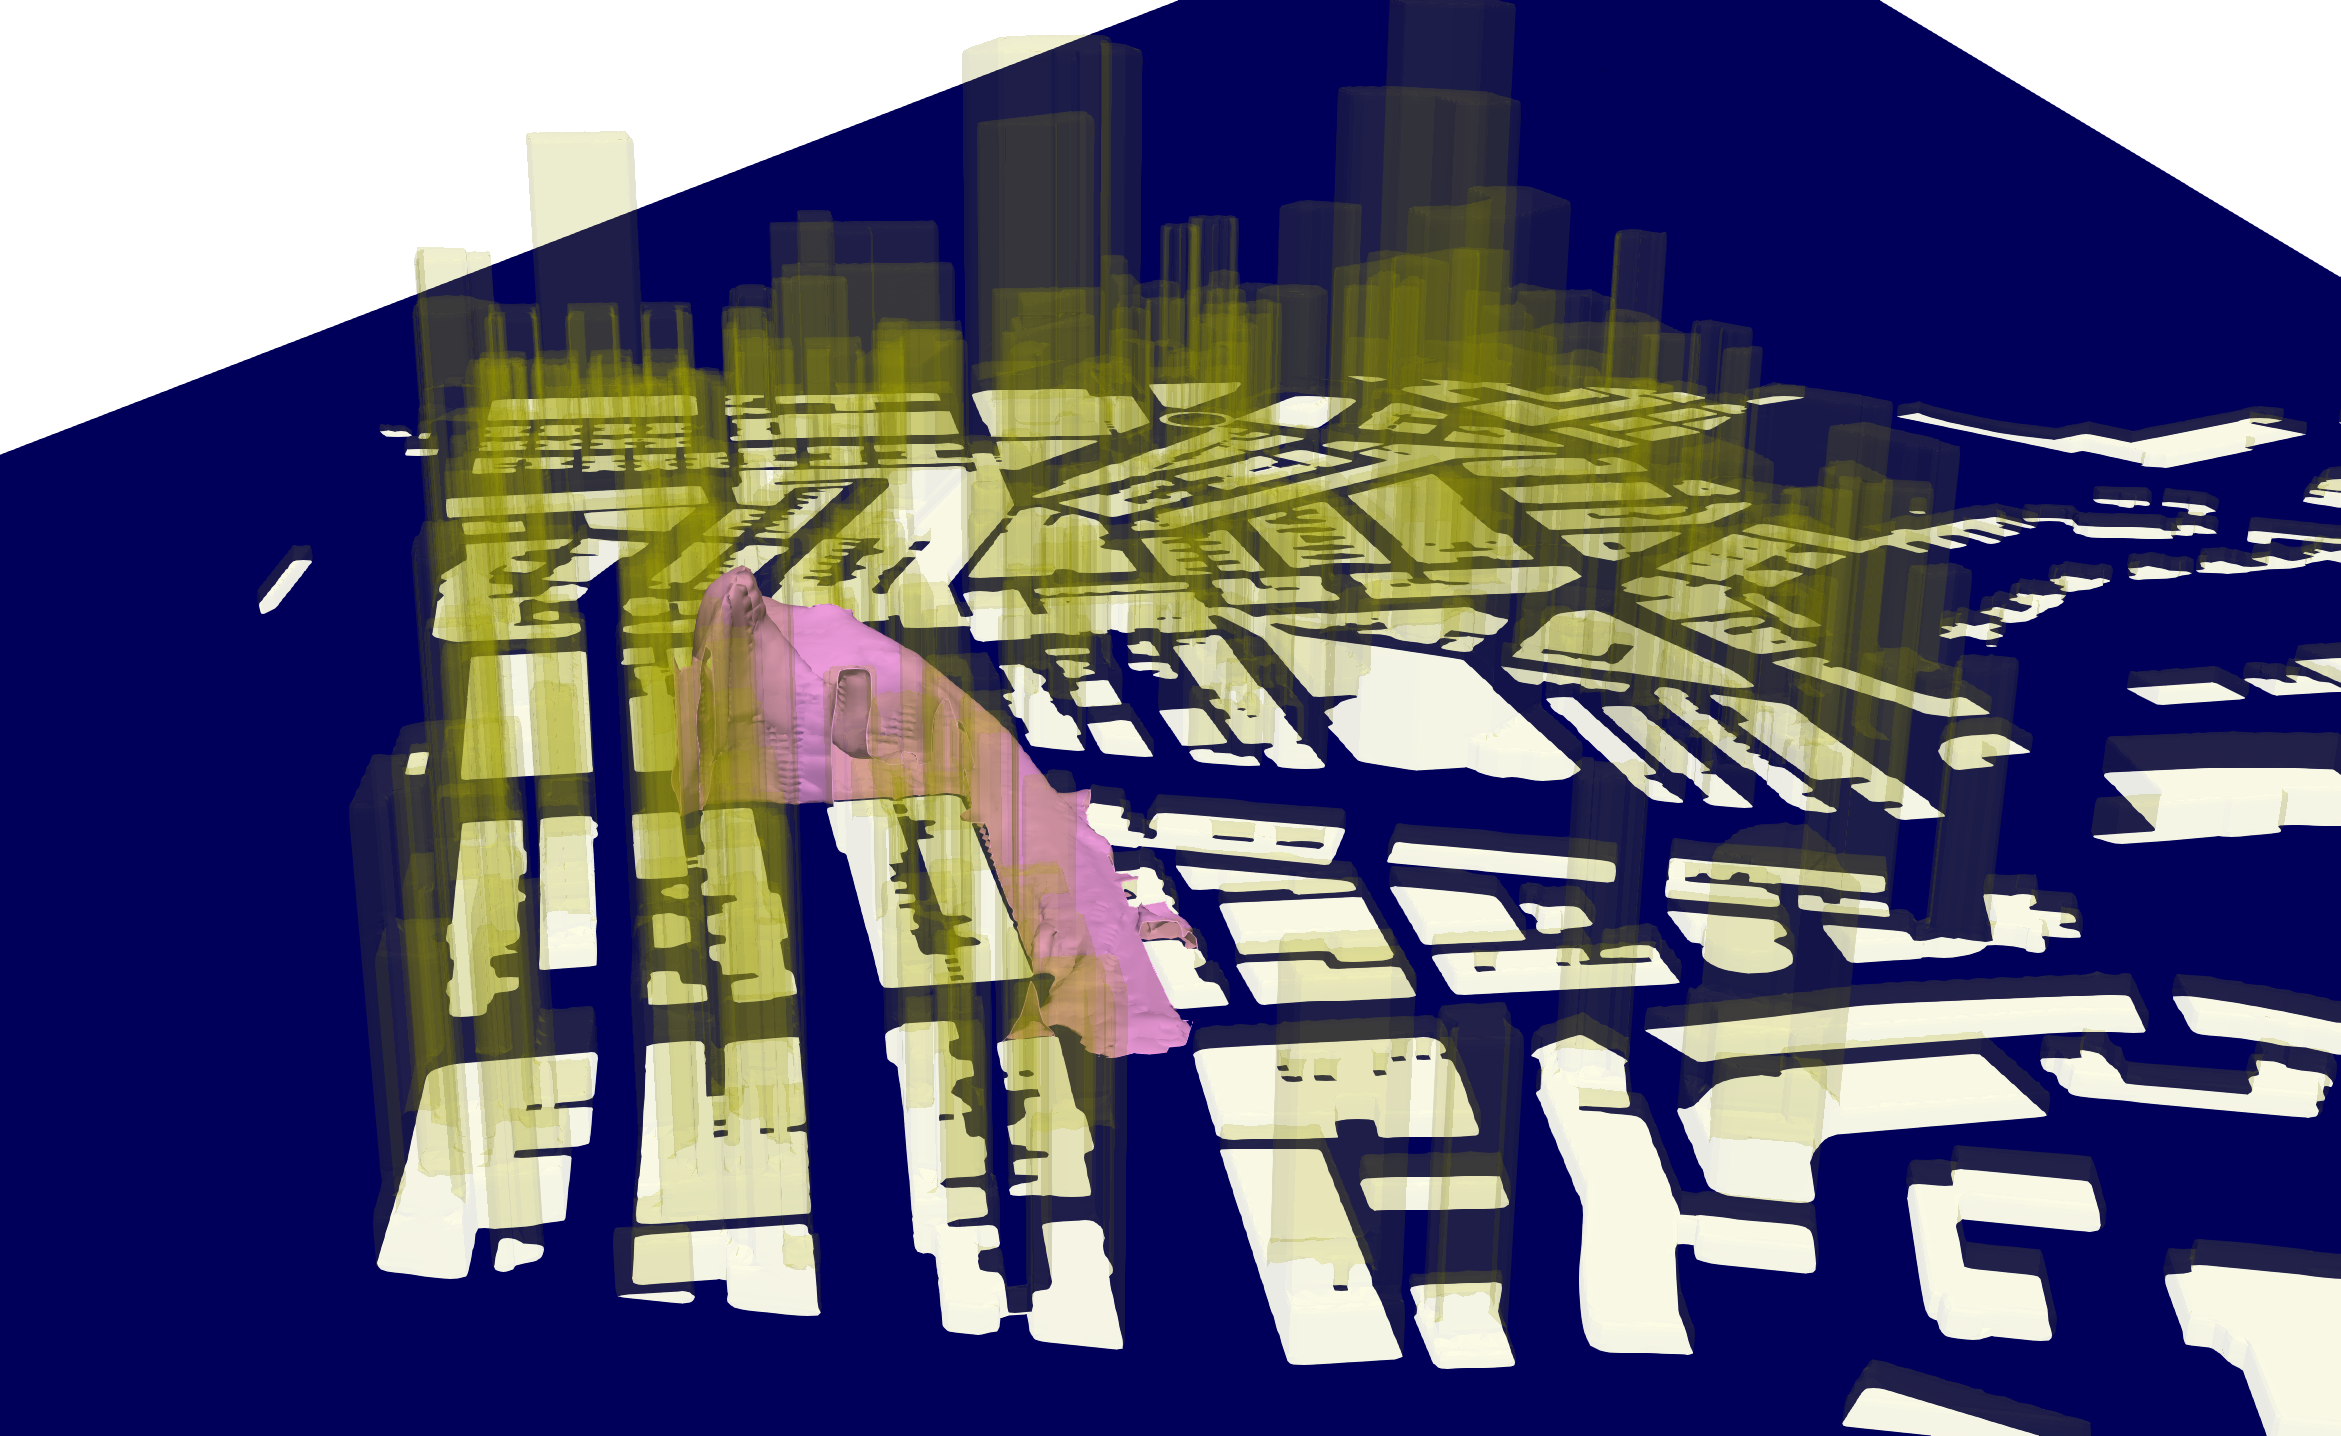
\includegraphics[width = 0.5\textwidth, trim={0 50px 0 200px},clip]{01_images/anim/animV1.0007.png}};
        \node at (right.west) [anchor=north, xshift = 0.2cm, rotate=90, color=white] {$t$ = 50\,s};
        % \node (right) at (left.east) [anchor=west] {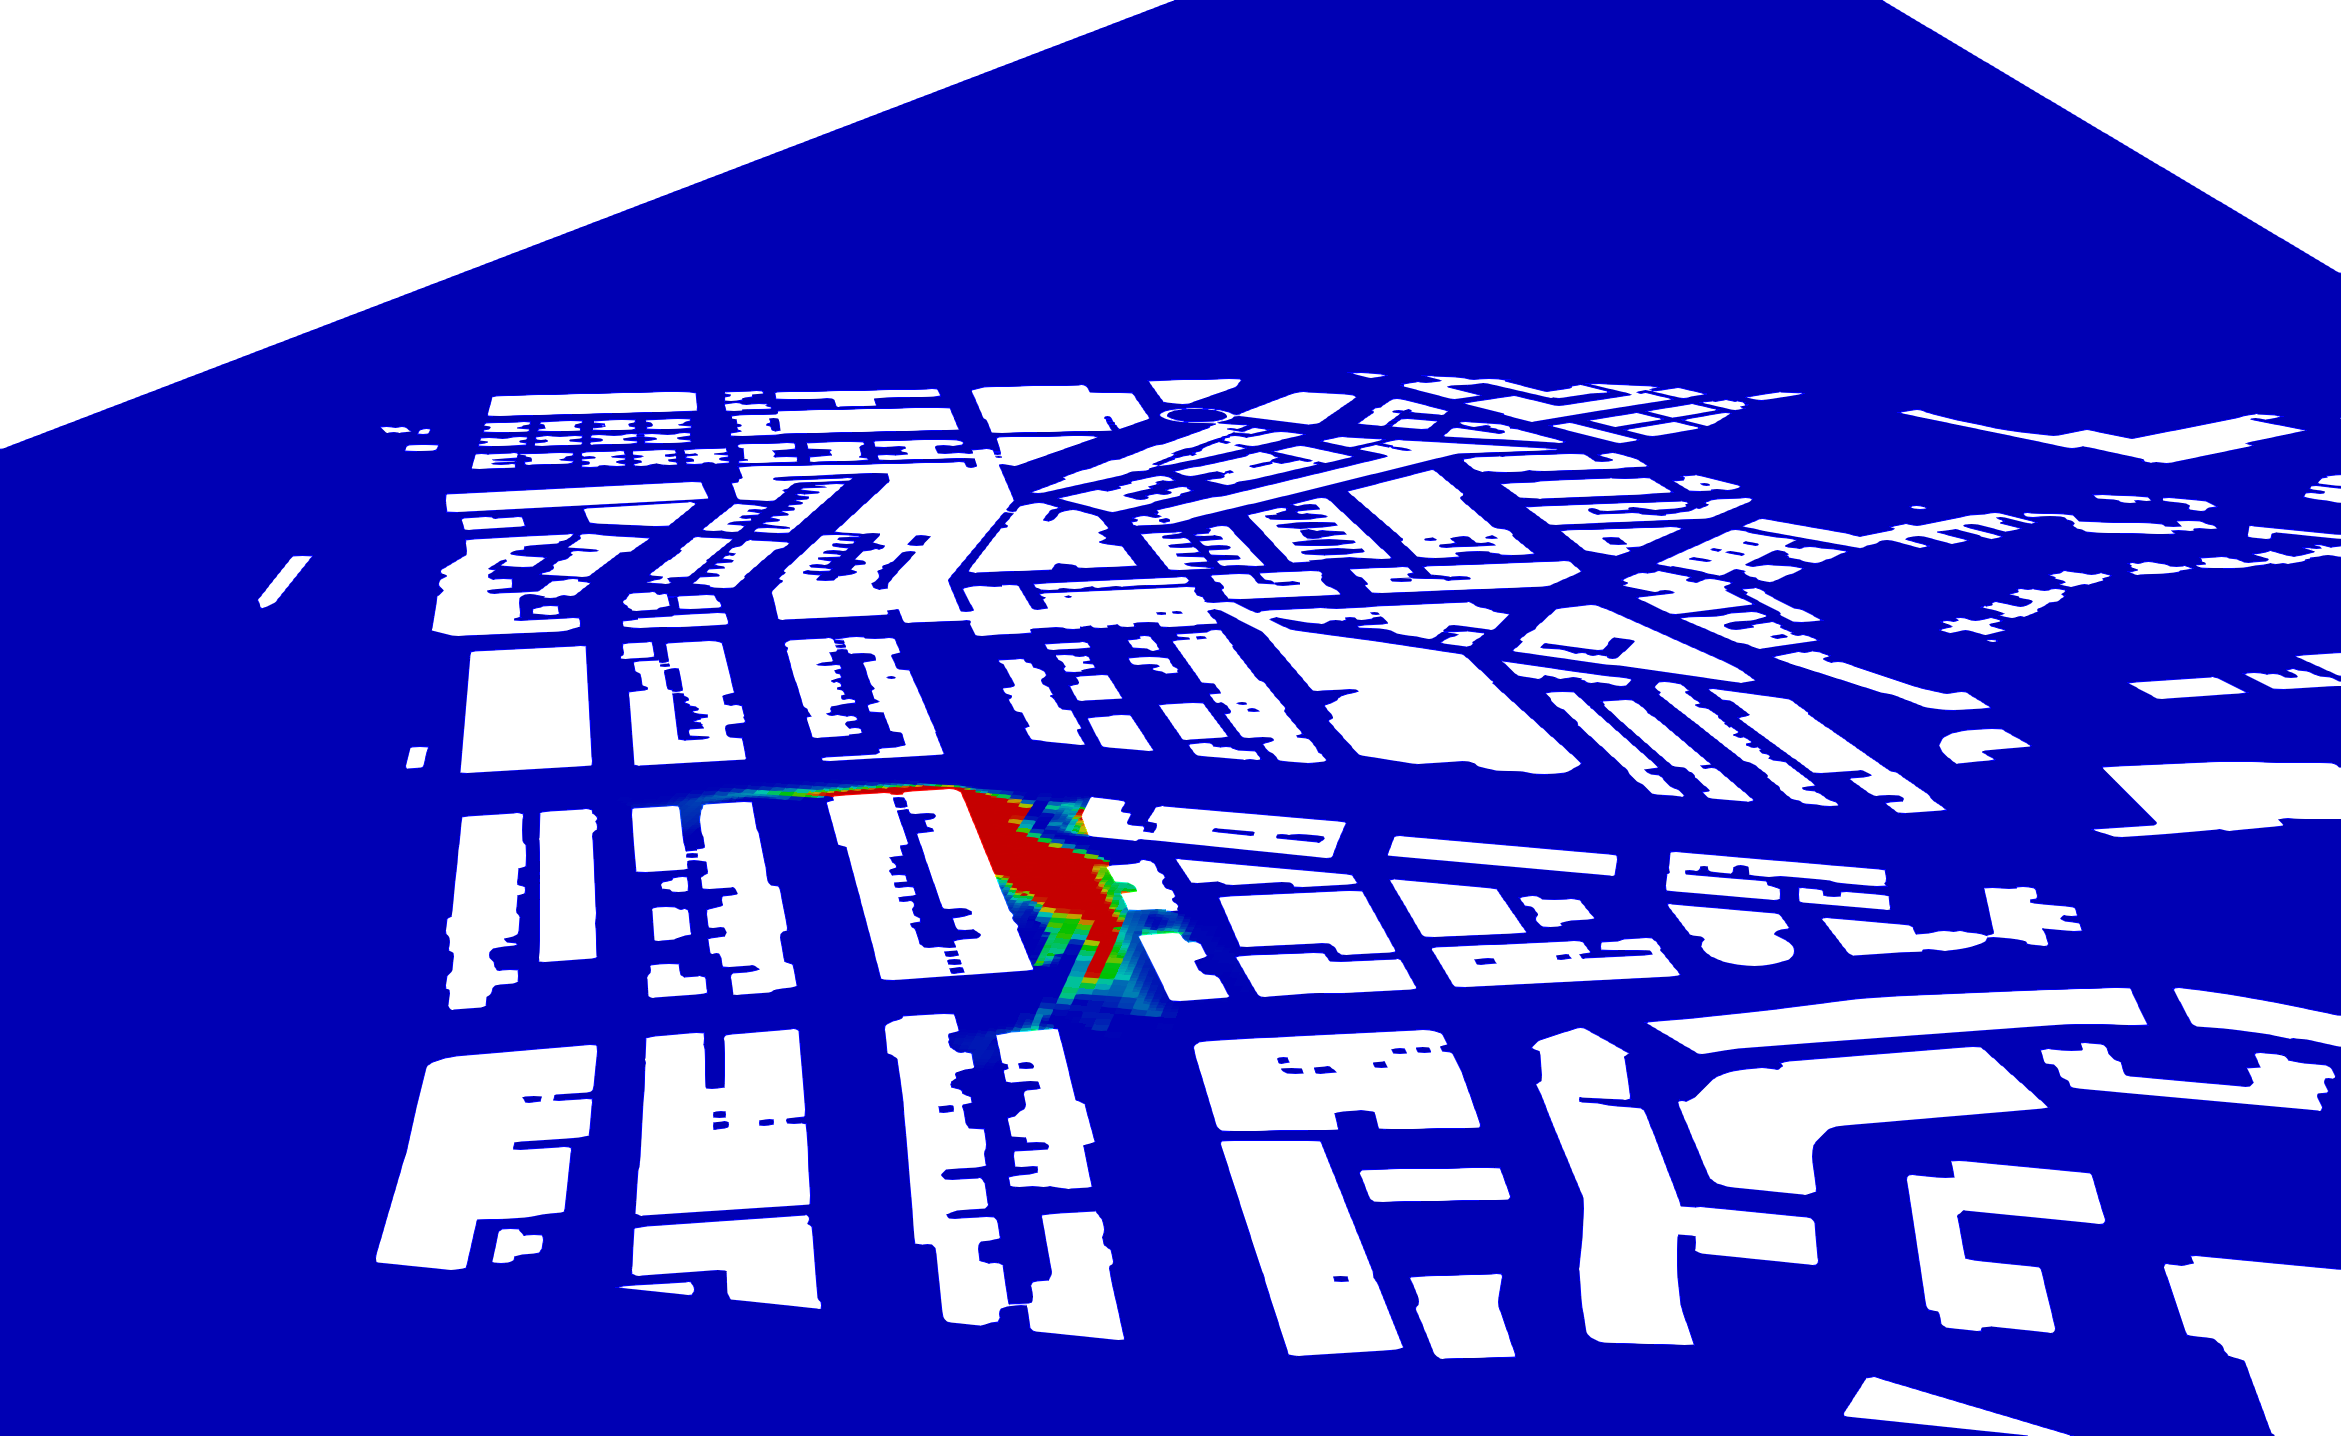
\includegraphics[width=0.23\textwidth, trim={500px 50px 1000px 200px},clip]{01_images/anim2/animV1.0005.png}};
        \node (left) at (left.south) [anchor=north] {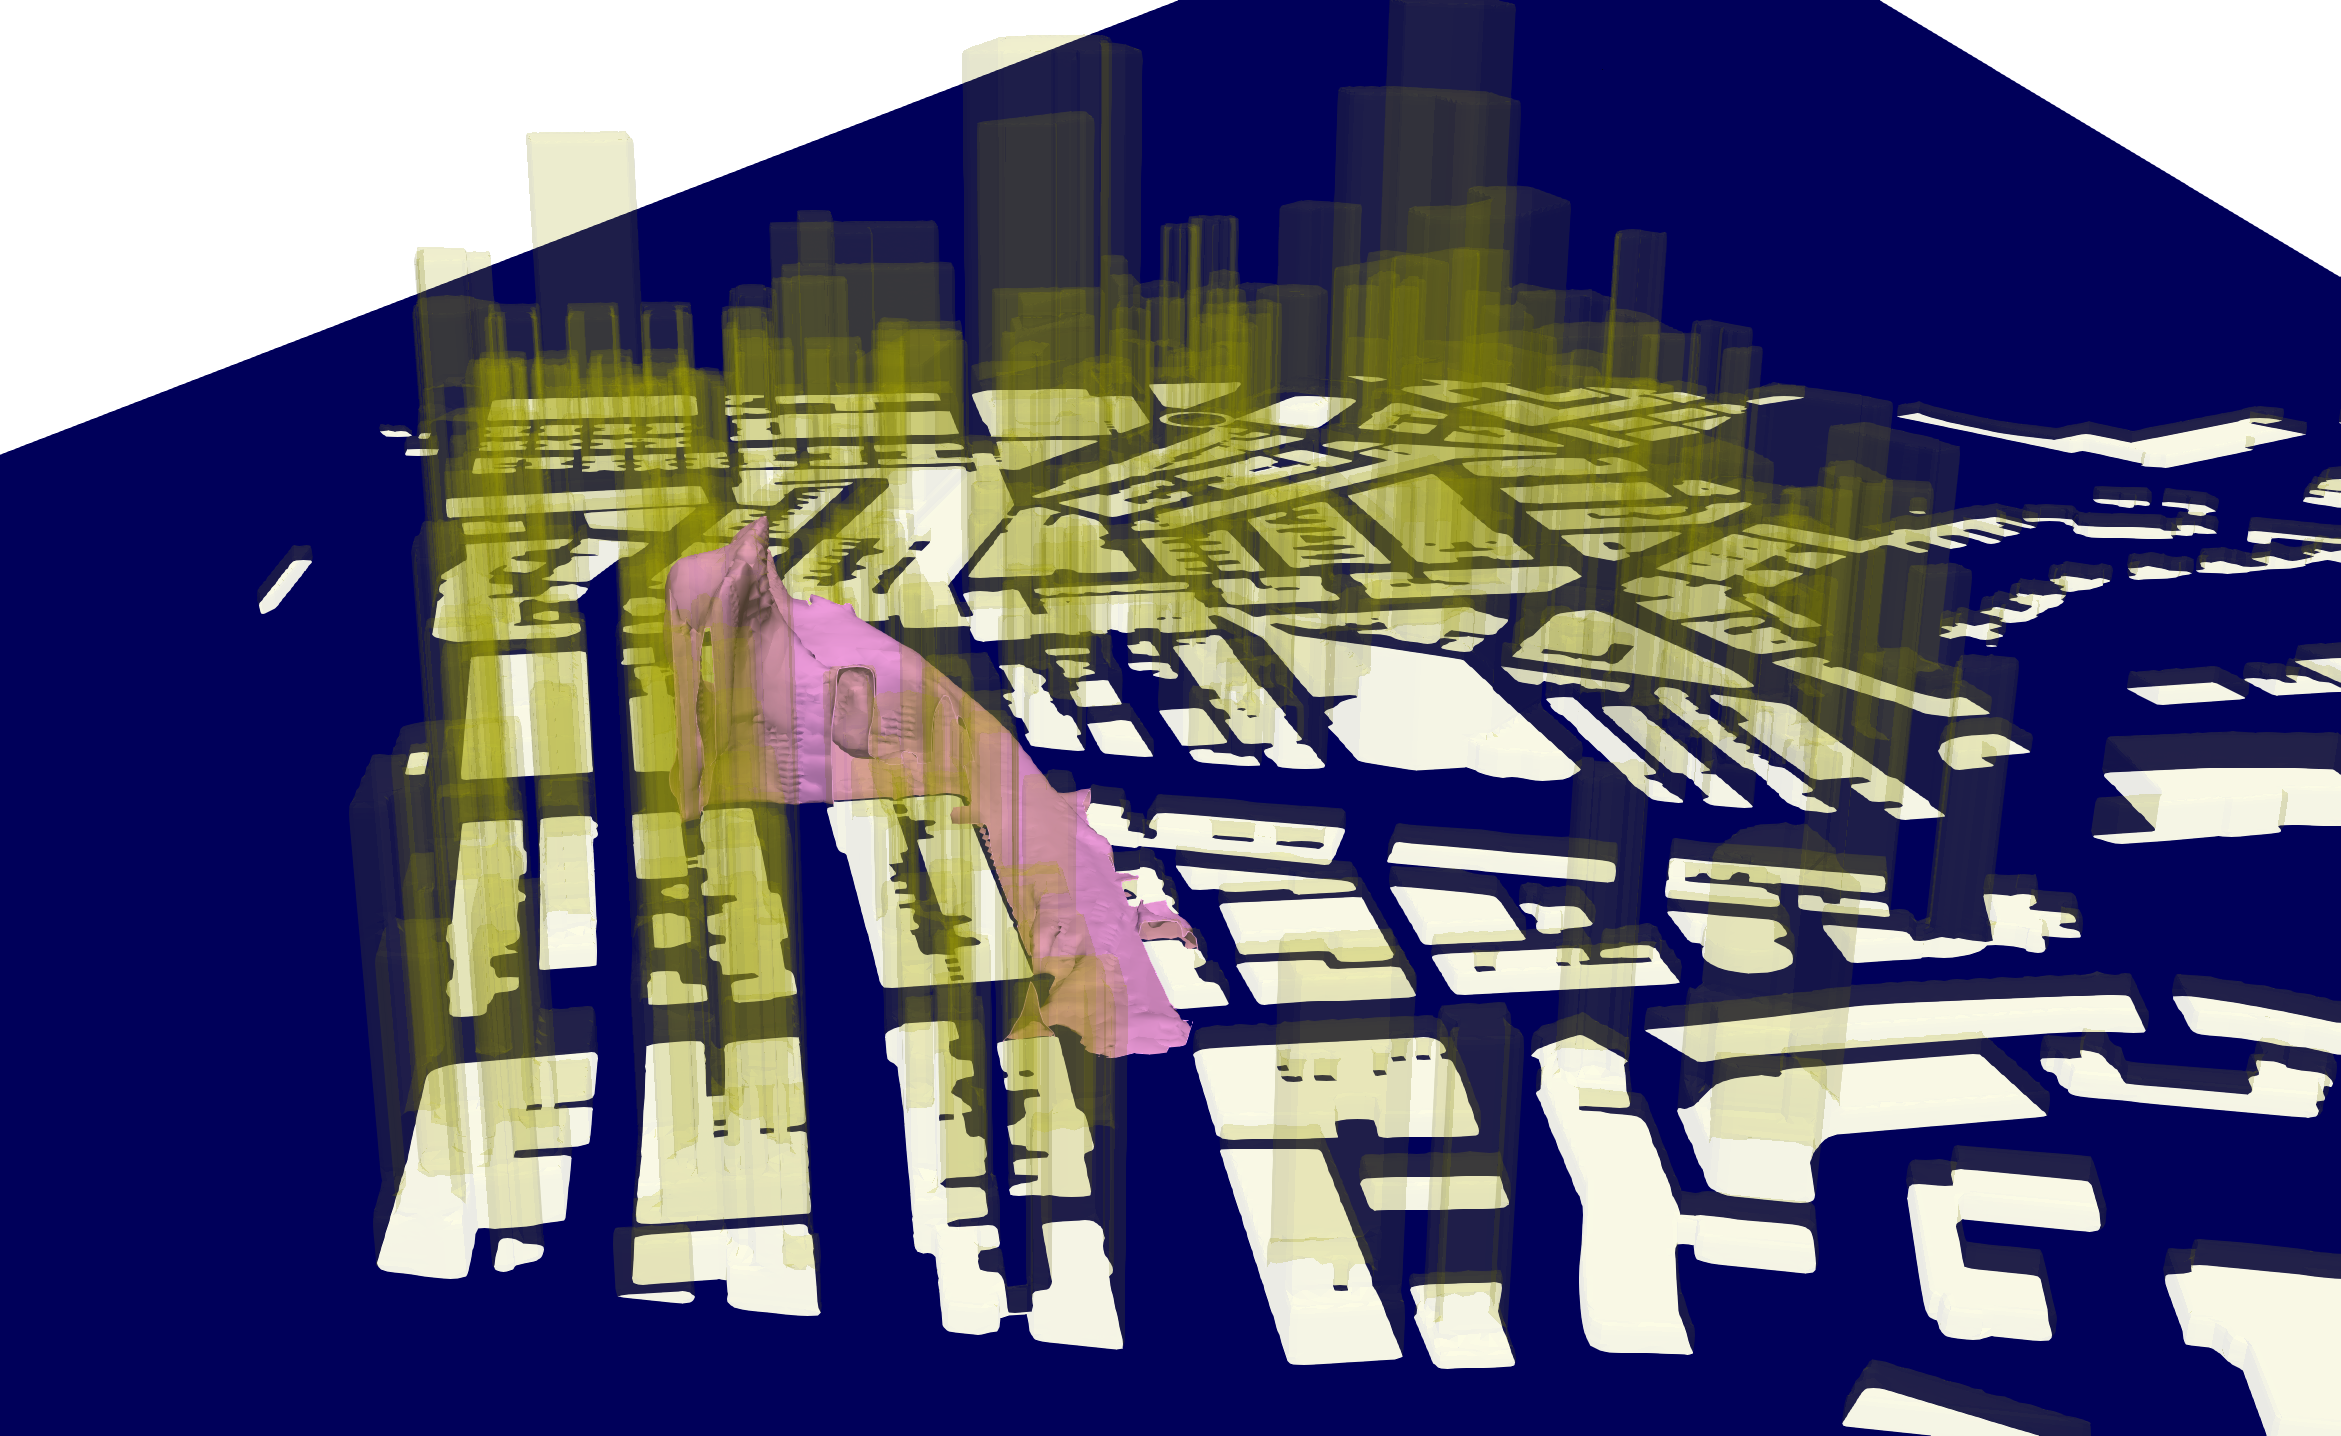
\includegraphics[width = 0.5\textwidth, trim={0 50px 0 200px},clip]{01_images/anim/animV1.0008.png}};
        \node at (left.west) [anchor=north, xshift = 0.2cm, rotate=90, color=white] {$t$ = 60\,s};
        \node (right) at (left.east) [anchor=west] {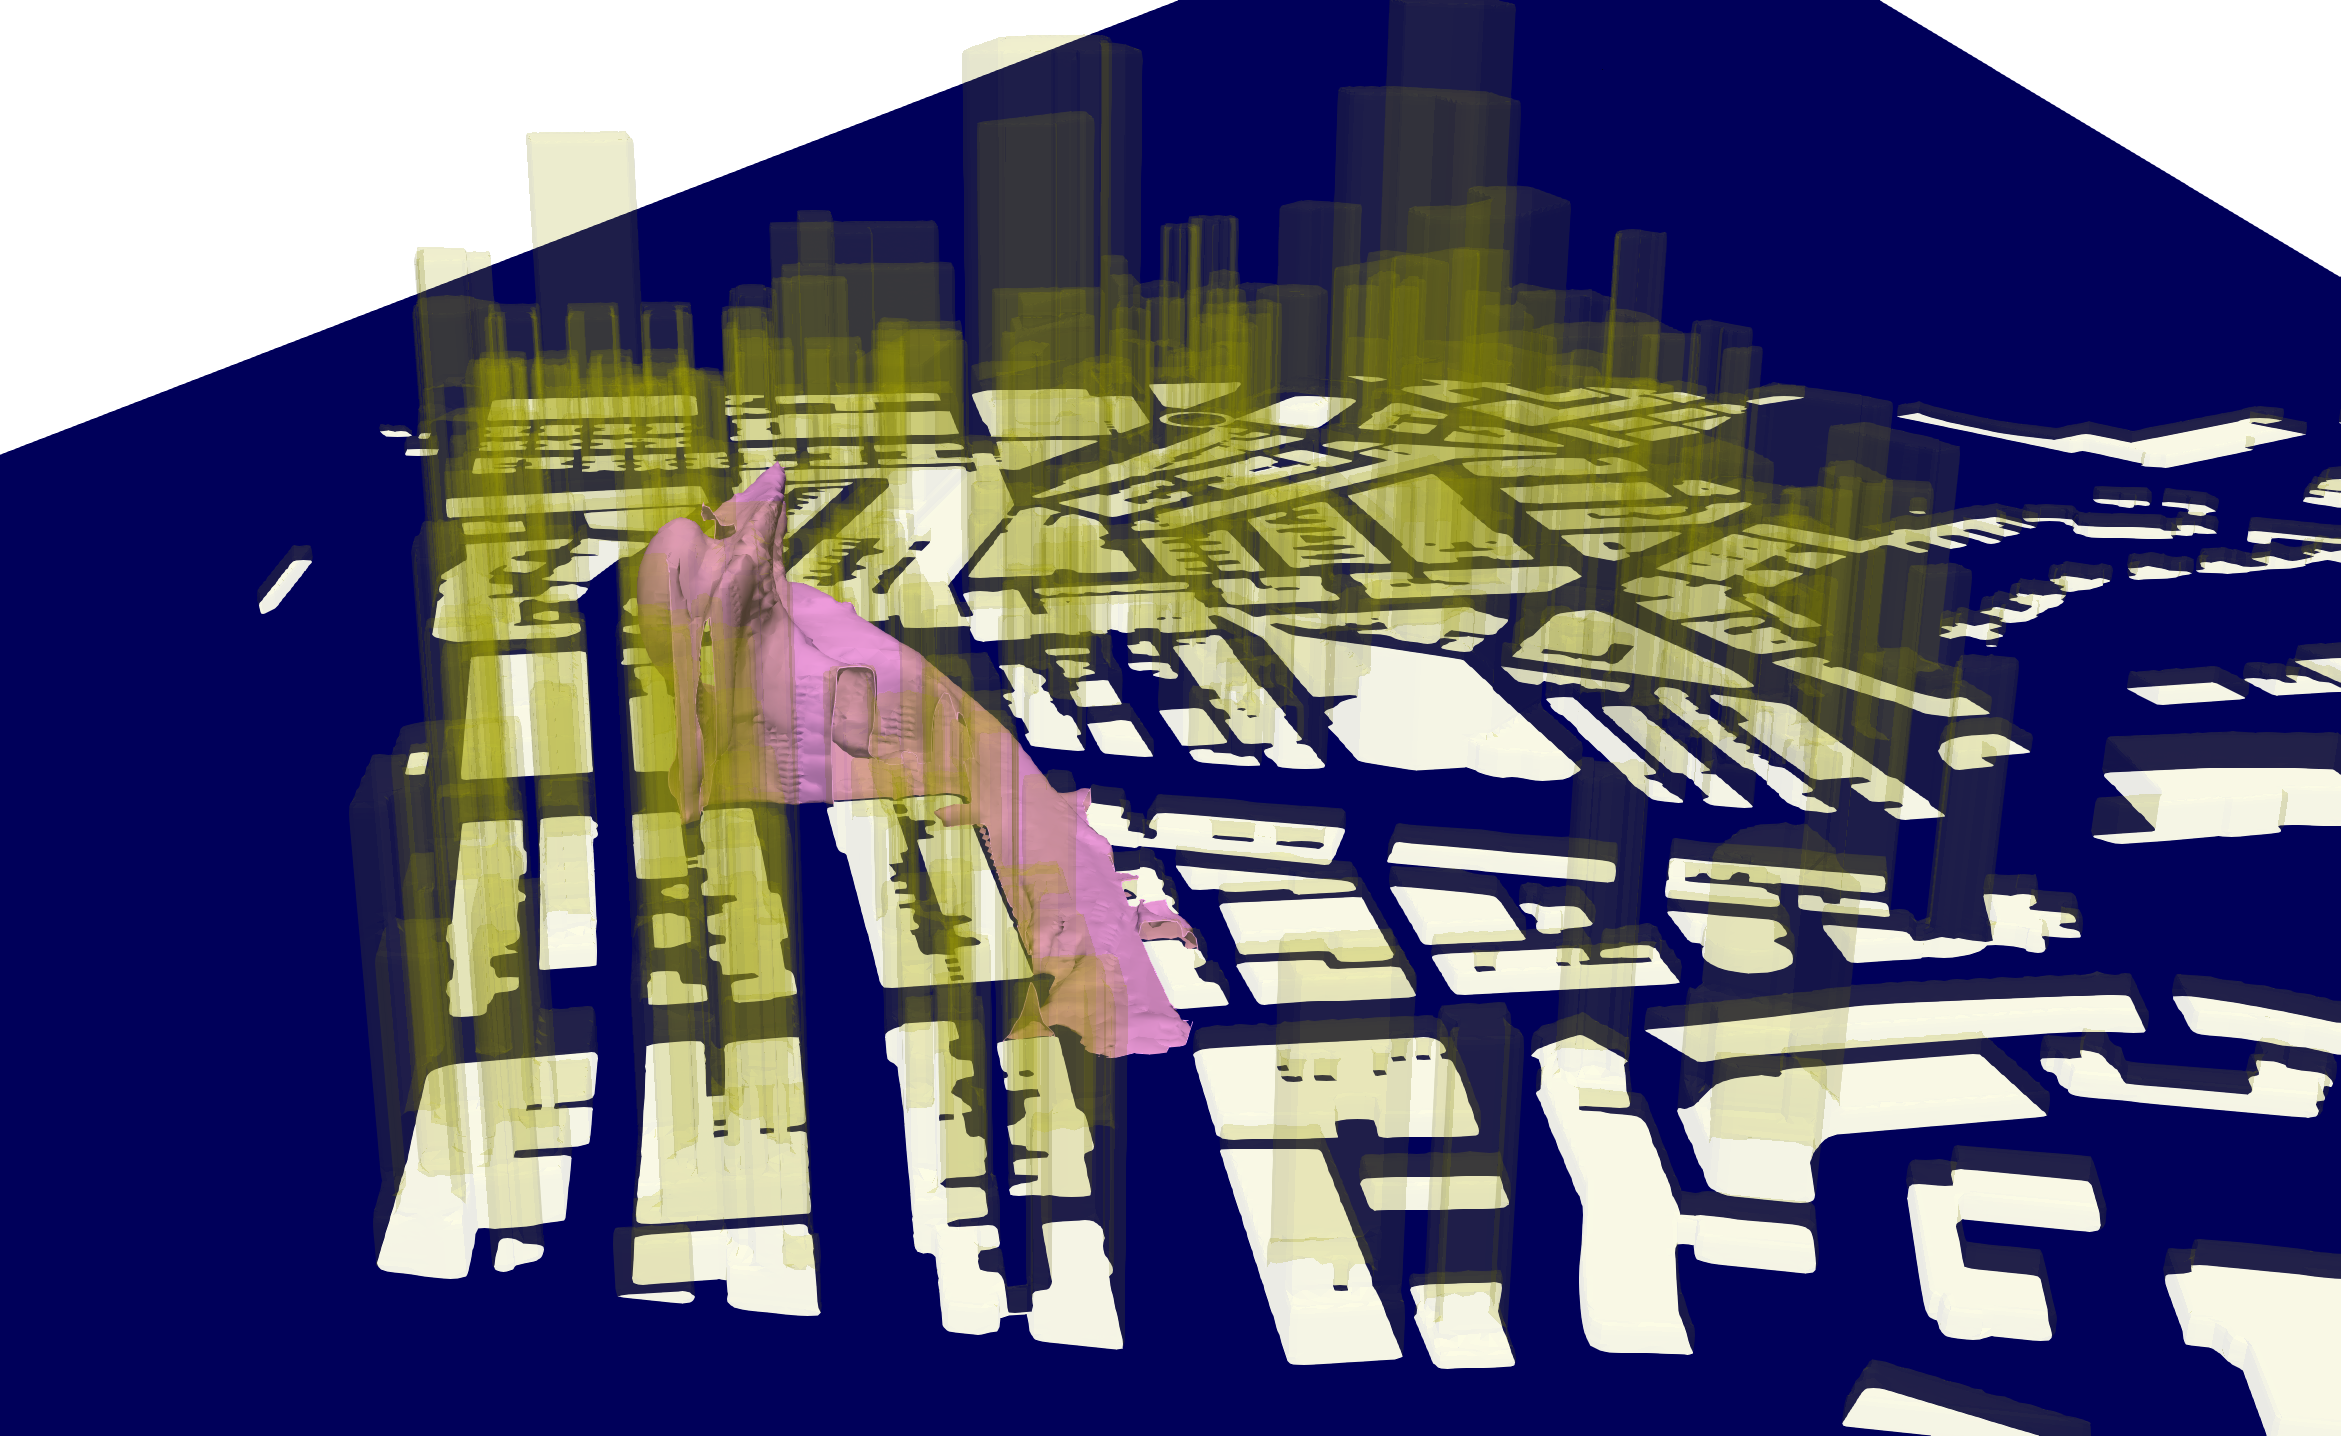
\includegraphics[width = 0.5\textwidth, trim={0 50px 0 200px},clip]{01_images/anim/animV1.0009.png}};
        \node at (right.west) [anchor=north, xshift = 0.2cm, rotate=90, color=white] {$t$ = 70\,s};
        % \node (right) at (left.east) [anchor=west] {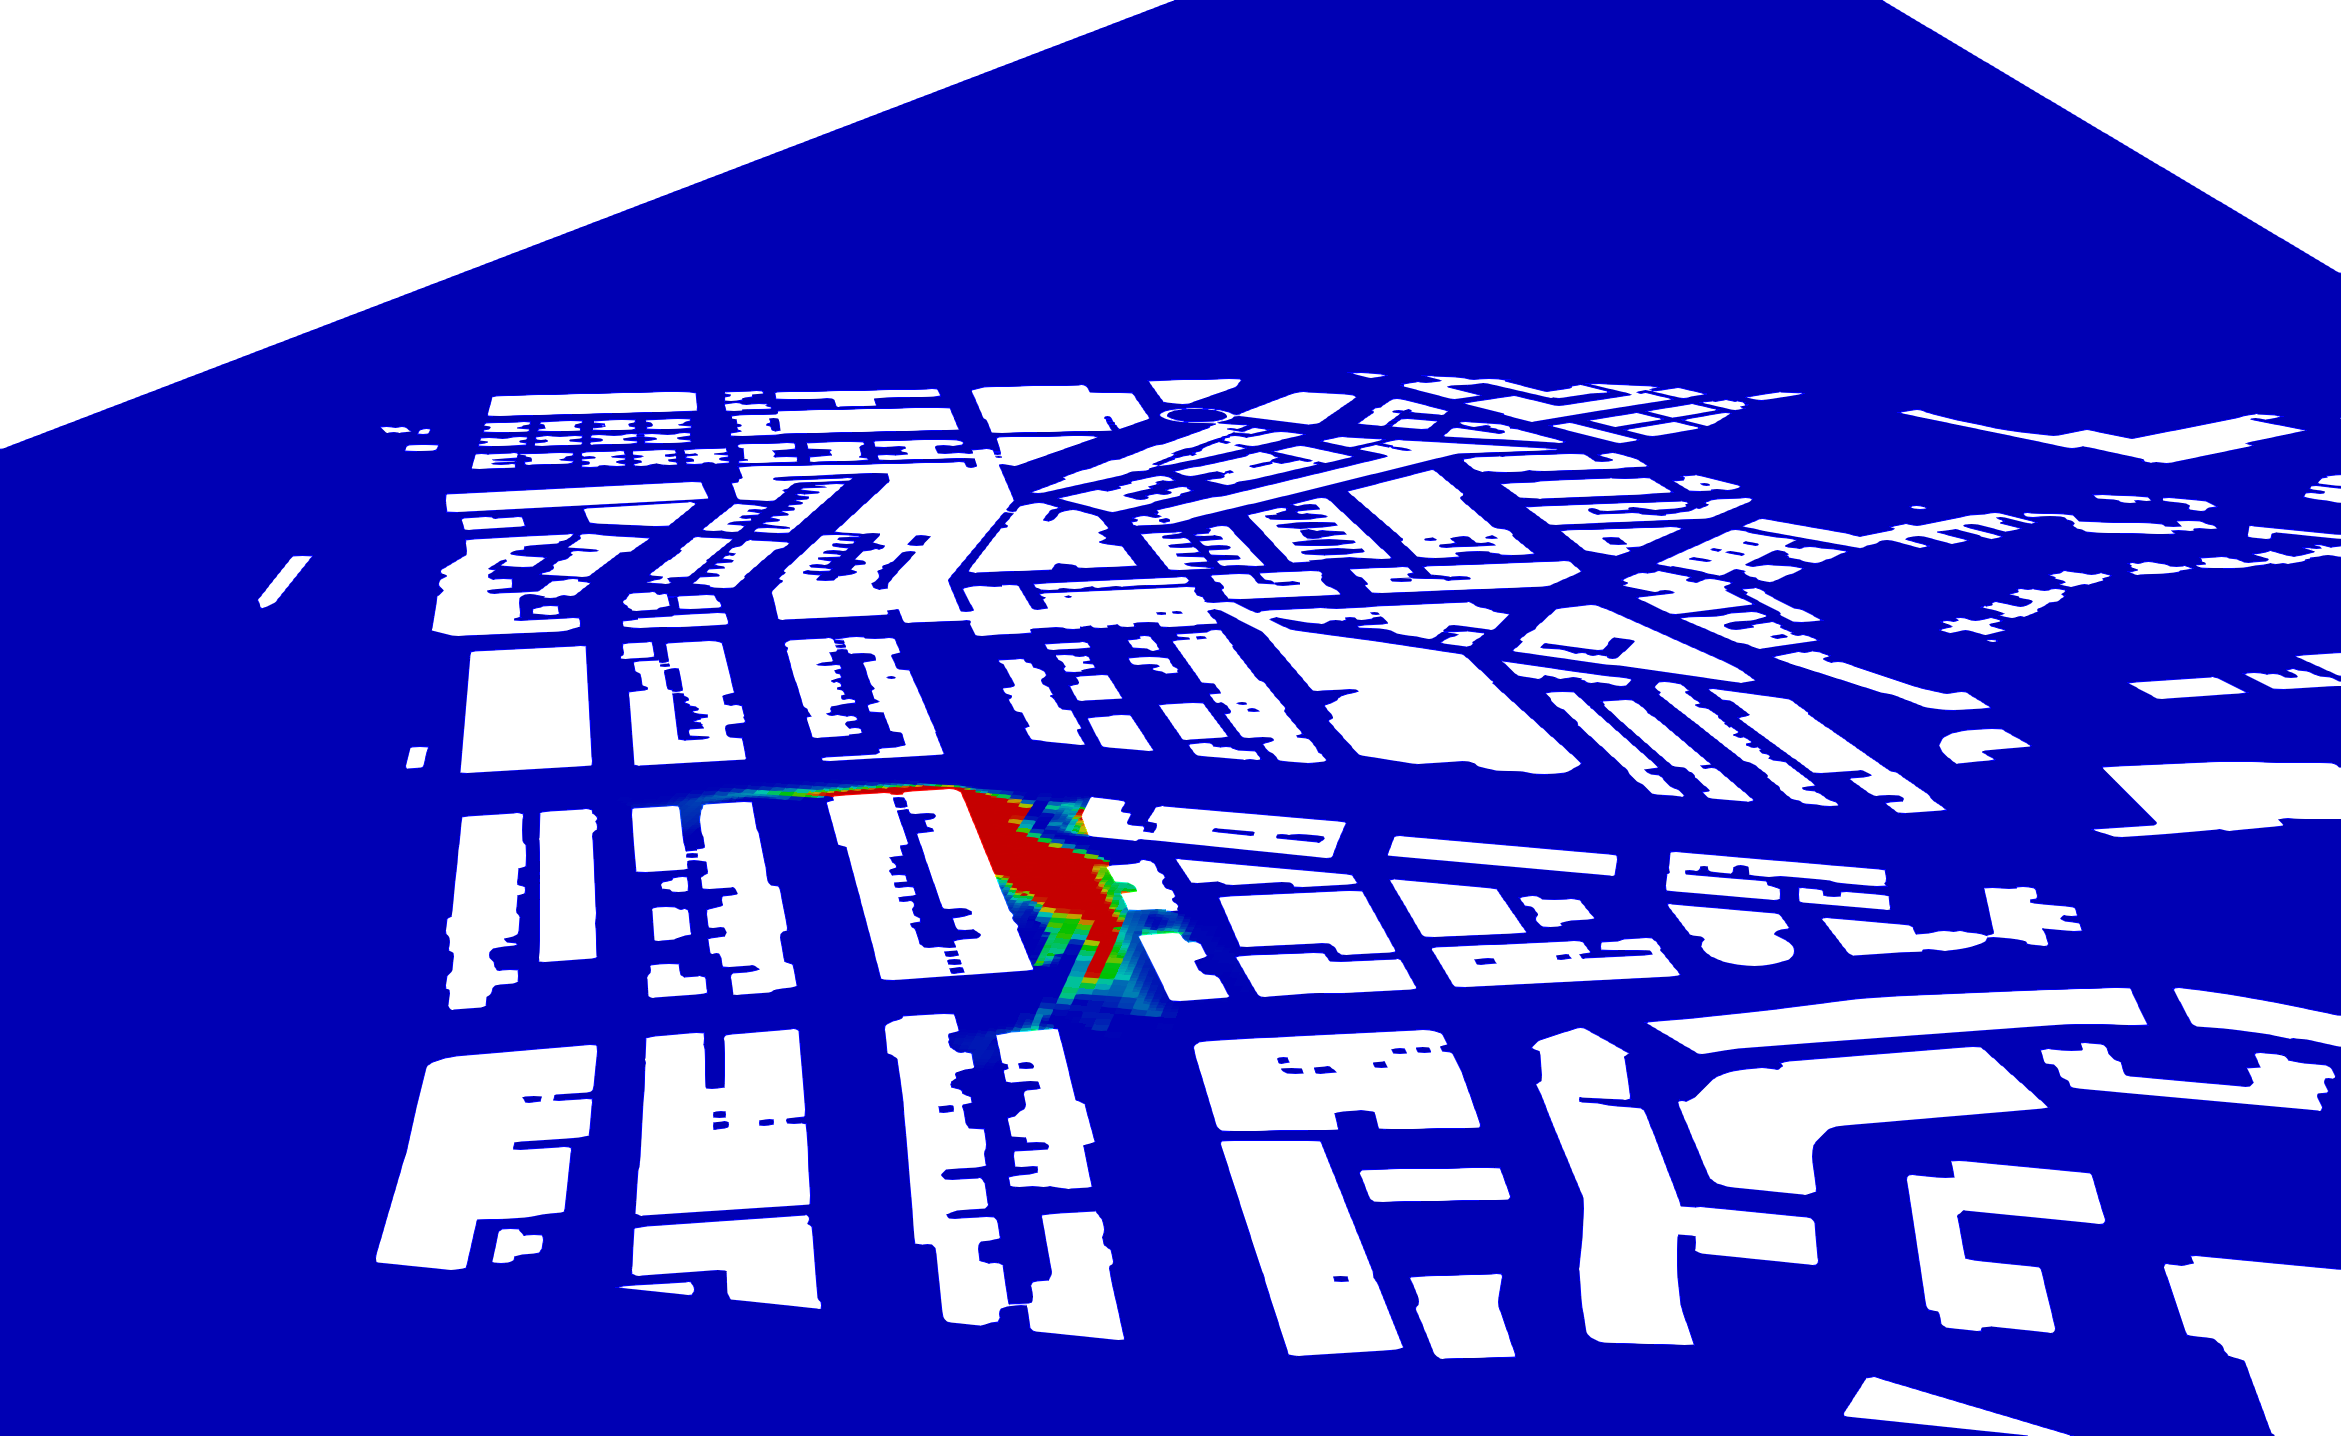
\includegraphics[width=0.23\textwidth, trim={500px 50px 1000px 200px},clip]{01_images/anim2/animV1.0005.png}};
    \end{tikzpicture}
    \caption{Time development of the air pollution spreading inside city, contour $y_{\mathrm{pol}}\,=\,1\,$ppm in pink.}
    \label{fig:pol}
\end{figure}

Next, main flow pathways are visualized utilizing the flow streamlines colored by the streamwise velocity component in Figure~\ref{fig:ux_p}b.

Steady-state velocity field obtained by the solution of~(\ref{eq:RANS1},~\ref{eq:RANS2}) can be used in the simulation of the pollution spreading, which is assumed transient. The resulting time development of the pollution at street is visualized by $y_{\mathrm{pol}}\,=\,1\,$ppm contour colored by pink in Figure~\ref{fig:pol} for times $t\,=\,$1, 10, 20, 30, 40, 50, 60, and 70\,s.